\ifx\wholebook\relax\else
\documentclass[twoside]{book}
\usepackage[active]{srcltx}
\usepackage[LY1]{fontenc}
\usepackage{epsfig}
\def\etc{{\it etc}}
\def\eg{{\it e.g.}}
\def\ie{{\it i.e.}}
\def\cf{{\it c.f.}\ }
\def\erf{\mathop{\rm erf}}
\def\sign{\mathop{\rm sign}}
\def\prob{\mathop{\rm Prob}}
\def\var{\mathop{\rm var}}
\def\mod{\mathop{\rm mod}}
\def\cor{\mathop{\rm cor}}
\def\cov{\mathop{\rm cov}}
\def\cl{\mathop{\rm CL}}
\def\kg{\mathop{\rm Kg}}
\def\patstyle#1{{\sc #1}}
\def\th{^{\mathop{\rm th}}}
\def\st#1{^{\mathop{\rm #1}}}
\def\note#1{\begin{quote}{\bf Note:} #1\end{quote}}
\def\braket#1{\left\langle #1\right\rangle}
\def\order#1{\let\o=#1{\cal O}\ifx\o 1$\left(n\right)$\else$\left(n^{#1}\right)$\fi}
\newtheorem{privListing}{Listing}[chapter]
\newenvironment{listing}{\vskip 3ex\hrule\vskip 1ex\begin{privListing}}{\end{privListing}\hrule\vskip 1ex}
\newtheorem{privExample}{Code example}[chapter]
\newenvironment{codeExample}{\begin{privExample}\begin{quote}\tt}{\end{quote}\end{privExample}}
\def\relboxl#1#2{\hbox to #1\hsize{#2\hfil}}
\def\relboxc#1#2{\hbox to #1\hsize{\hfil #2\hfil}}
\def\relboxr#1#2{\hbox to #1\hsize{\hfil #2}}
\def\transpose#1{{\bf #1}^{\mathop{\rm T}}}
\def\inverse#1{{\bf #1}^{-1}}
%\def\tm{$^{\mathop{\rm TM}}$}
\def\tm{ }
\newenvironment{mainEquation}{\marginpar[\vspace{3 ex} Main
equation$\Rightarrow$]{\vspace{3 ex}$\Leftarrow$Main
equation}\begin{equation}}{\end{equation}}
\def\rubrique#1{\paragraph{#1}\hfil\par\noindent}

\begin{document}
\fi

\chapter{Additional probability distributions}
\label{ch:distributions}

\section{Beta distribution}
\label{sec:betadist} Table \ref{tb:betadist} shows the properties
of the beta distribution.
\begin{table}[h]
  \centering
  \caption{Properties of the beta distribution}\label{tb:betadist}
\vspace{1 ex}
\begin{tabular}{|l|c|} \hline
  \vbox to 3ex{}Range of random variable & $\left[0,1\right]$\\ *[1ex] \hline
  \vbox to 4ex{}Probability density function & $\displaystyle P\left(x\right)={1\over B\left(\alpha_1,\alpha_2\right)}
  x^{\alpha_1 - 1}\left(1-x\right)^{\alpha_2 - 1}$ \\*[2ex]  \hline
  \vbox to 3ex{}Parameters & $0<\alpha_1<+\infty$ \\
  & $0<\alpha_2<+\infty$\\*[1ex]  \hline
  \vbox to 4ex{}Distribution function & $\displaystyle F\left(x\right)=B\left(x;\alpha_1,\alpha_2\right)$ \\
  &(\cf section \ref{sec:incbeta}) \\*[1ex]  \hline
  \vbox to 3ex{}Average & $\displaystyle{\alpha_1 \over \alpha_1+\alpha_2}$ \\*[2ex] \hline
  \vbox to 4ex{}Variance & $\displaystyle{\alpha_1 \alpha_2
   \over \left(\alpha_1+\alpha_2\right)^2\left(\alpha_1+\alpha_2+1\right)}$ \\*[3ex] \hline
  \vbox to 4ex{}Skewness & $\displaystyle 2{\alpha_1 - \alpha_2
   \over \left(\alpha_1+\alpha_2+2\right)}$ \\*[3ex] \hline
  \vbox to 4ex{}Kurtosis & \parbox{8cm}{$$\begin{array}{l}\displaystyle{\root 3 \of {\alpha_1+\alpha_2+2
  \over \alpha_1 \alpha_2}} \left\{ {\left(\alpha_1+\alpha_2+1\right)
  \over \alpha_1 \alpha_2
  \left(\alpha_1+\alpha_2+2\right)
  \left(\alpha_1+\alpha_2+3\right)}\right.\\*[4ex]
  \qquad \times \left.\left[2\left(\alpha_1+\alpha_2\right)^2+\alpha_1 \alpha_2
  \left(\alpha_1+\alpha_2-6\right)\right]-1\right\}\end{array}$$} \\*[1ex] \hline
\end{tabular}
\end{table}
If the parameters $\alpha_1$ and $\alpha_2$ are equal to 1 the
beta distribution is identical to the uniform distribution over
the interval $\left[0,1\right]$.

The beta distribution is an ad-hoc distribution, which can take
many shapes. Figure \ref{fig:betaDistr} shows a few characteristic
shapes for several values of the parameters. The random variable
is limited to the interval $\left[0,1\right]$. However, any
distribution of a random variable varying over a finite interval
can be mapped to a beta distribution with a suitable variable
transformation.
\begin{figure}
\centering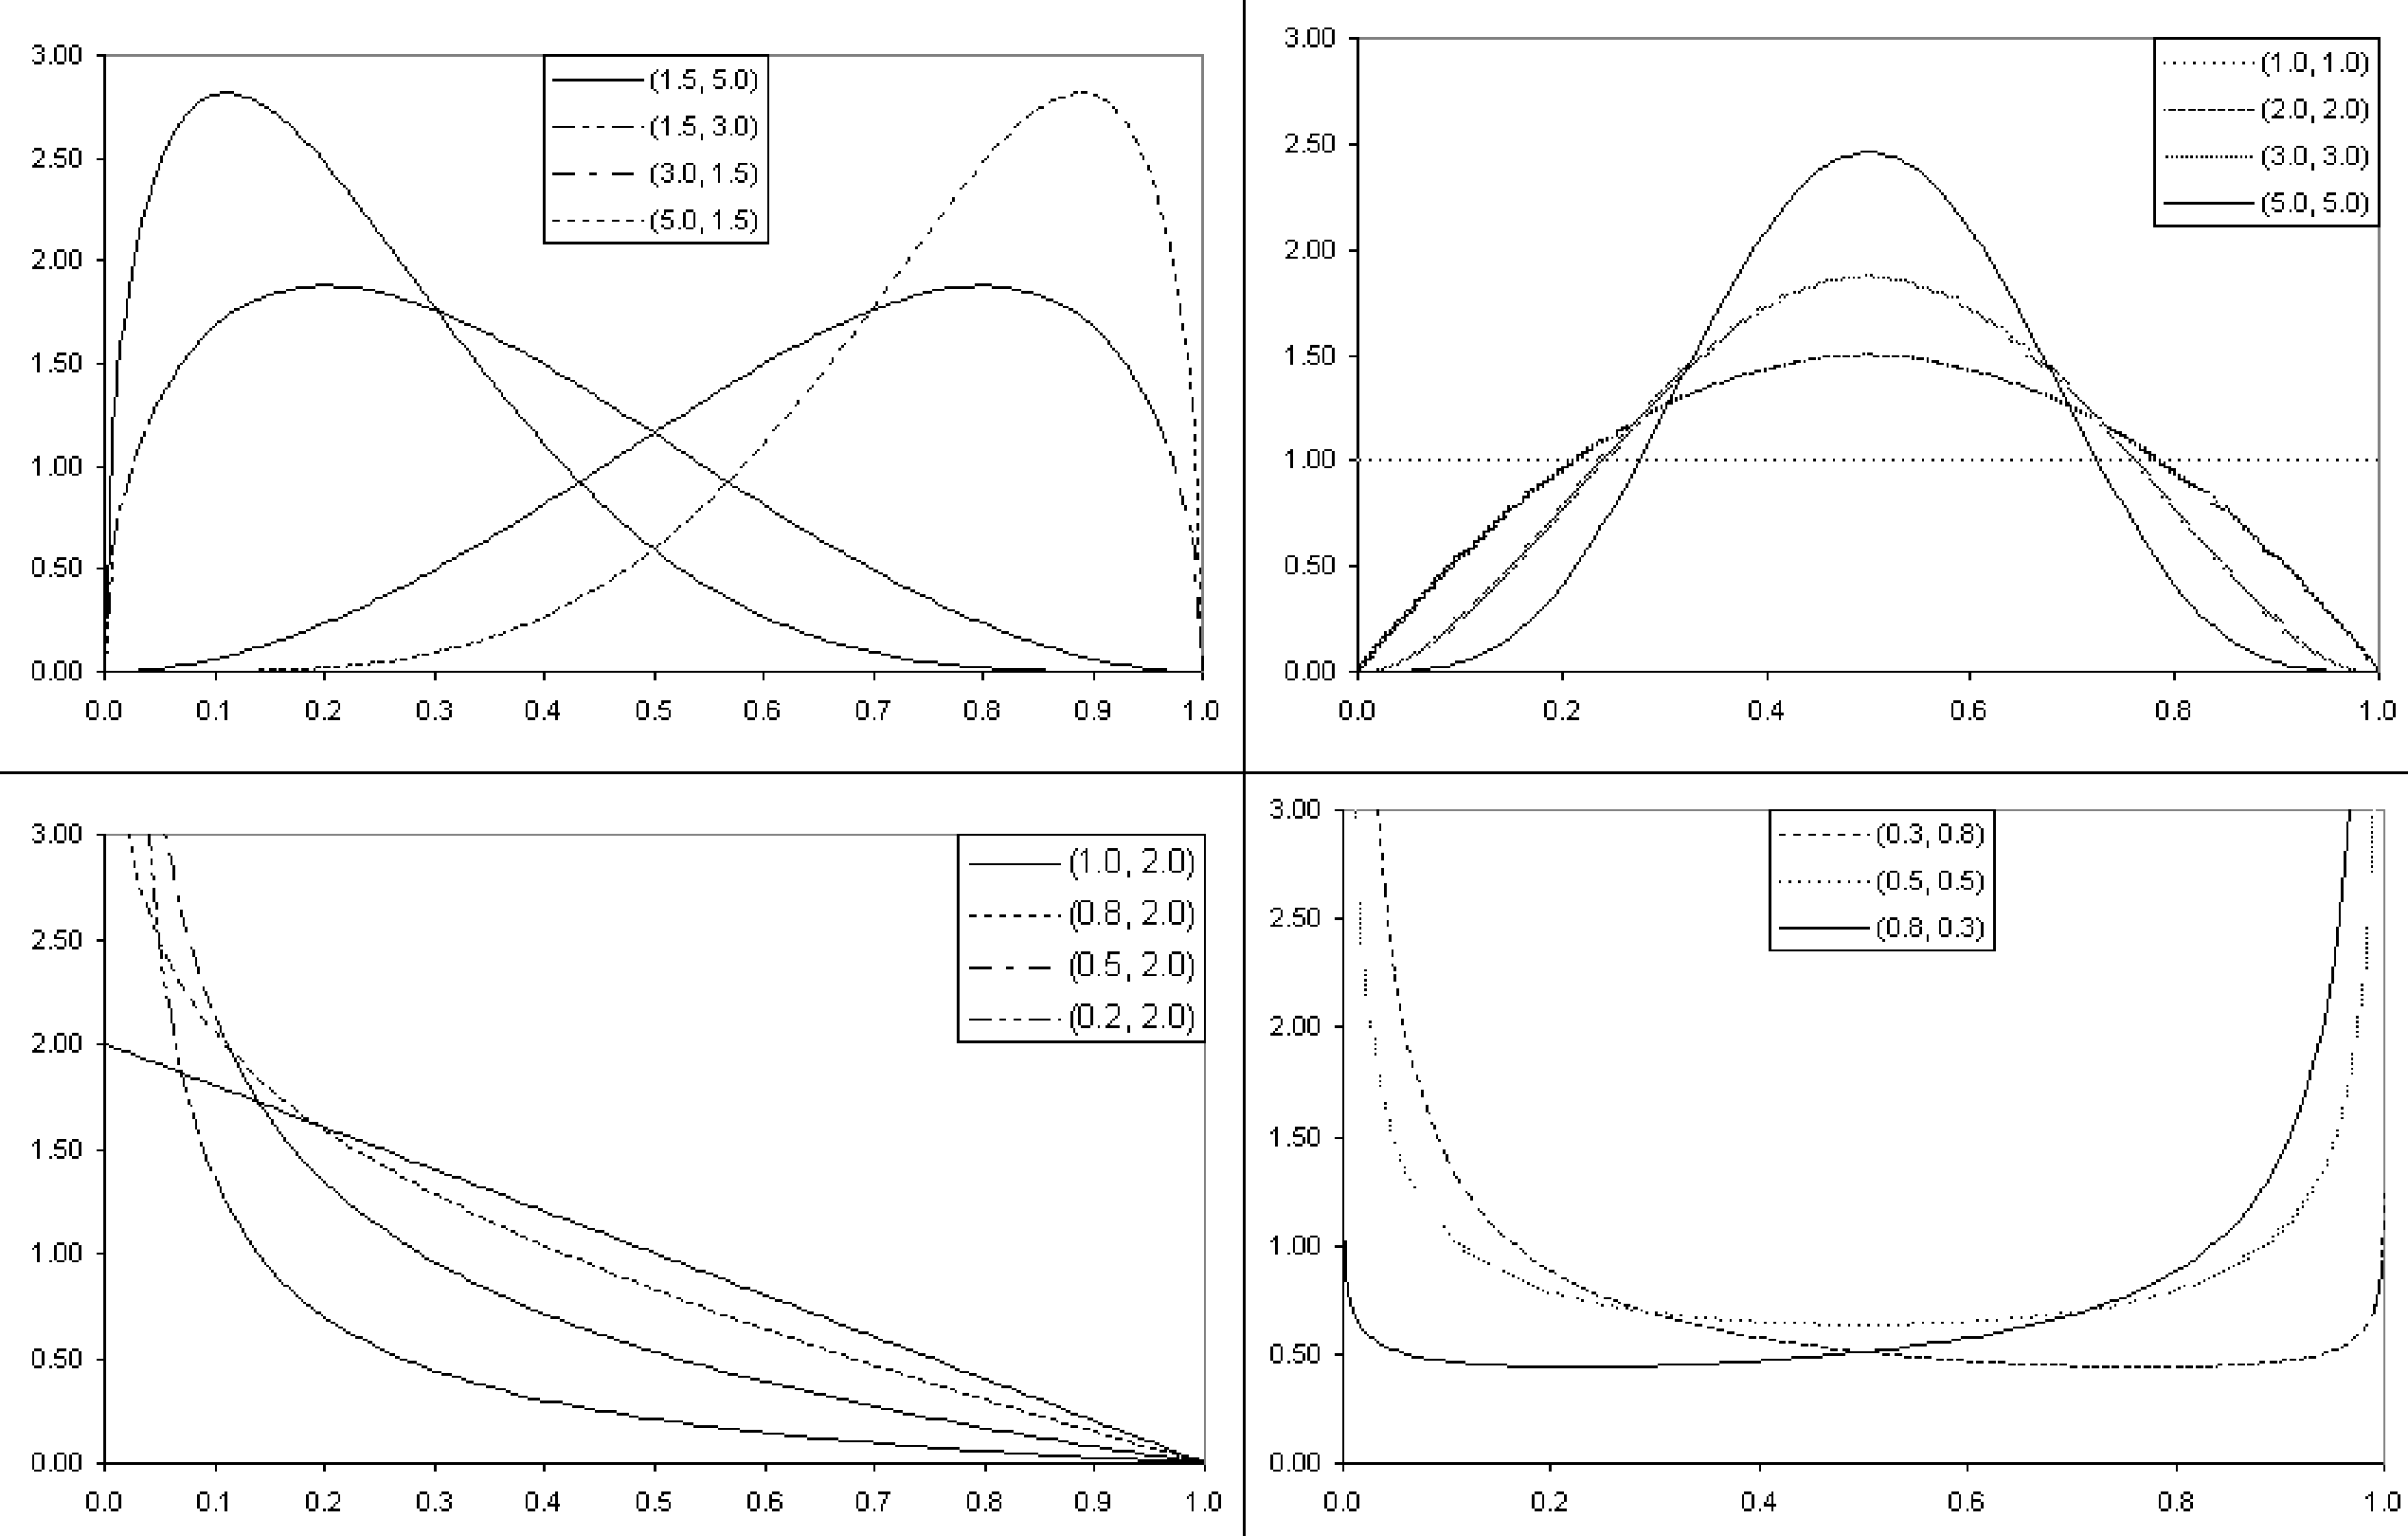
\includegraphics[width=12cm]{Figures/BetaDistribution}
\caption{Many shapes of the beta
distribution}\label{fig:betaDistr}
\end{figure}


\subsection{Beta distribution --- Smalltalk  implementation}
Listing \ref{ls:betadist} shows the implementation of the beta
distribution in Smalltalk.

\begin{listing} Smalltalk implementation of the beta distribution \label{ls:betadist}
$$\halign{ #\hfil&\quad#\hfil\cr {\sl Class}& {\Large\bf DhbBetaDistribution}\cr
{\sl Subclass of }&{\tt DhbProbabilityDensity}\cr\noalign{\vskip 1ex}

{\sl Instance variable names:}&\parbox[t]{4 in}{\tt  alpha1 alpha2 gamma1 gamma2 logNorm incompleteBetaFunction }\cr\noalign{\vskip 1ex}}$$


Class methods
{\parskip 1ex\par\noindent}
{\bf distributionName}
\begin{verbatim}
    ^'Beta distribution'

\end{verbatim}
{\bf fromHistogram:} {\tt aHistogram}
\begin{verbatim}
    | average variance a b c discr |
    ( aHistogram minimum < 0 or: [ aHistogram maximum > 1])
        ifTrue: [ ^nil].
    average := aHistogram average.
    variance := aHistogram variance.
    a := ( ( 1 - average) / variance - 1) * average.
    a > 0
        ifFalse:[ ^nil].
    b := ( 1 / average - 1) * a.
    b > 0
        ifFalse:[ ^nil].
    ^self shape: a shape: b

\end{verbatim}
{\bf new}
\begin{verbatim}
    ^self error: 'Illegal creation message for this class'

\end{verbatim}
{\bf shape:} {\tt aNumber1} {\bf shape:} {\tt aNumber2}
\begin{verbatim}
    ^super new initialize: aNumber1 shape: aNumber2

\end{verbatim}



Instance methods
{\parskip 1ex\par\noindent}
{\bf average}
\begin{verbatim}
    ^alpha1 / ( alpha1 + alpha2)

\end{verbatim}
{\bf changeParametersBy:} {\tt aVector}
\begin{verbatim}
    alpha1 := alpha1 + ( aVector at: 1).
    alpha2 := alpha2 + ( aVector at: 2).
    self computeNorm.
    gamma1 := nil.
    gamma2 := nil.
    incompleteBetaFunction := nil.

\end{verbatim}
{\bf computeNorm}
\begin{verbatim}
    logNorm := (alpha1 + alpha2) logGamma - alpha1 logGamma - alpha2 
                                                             logGamma.

\end{verbatim}
{\bf distributionValue:} {\tt aNumber}
\begin{verbatim}
    incompleteBetaFunction isNil
        ifTrue: [ incompleteBetaFunction := DhbIncompleteBetaFunction 
                                         shape: alpha1 shape: alpha2].
    ^incompleteBetaFunction value: aNumber

\end{verbatim}
{\bf firstGammaDistribution}
\begin{verbatim}
    gamma1 isNil
        ifTrue: [ gamma1 := DhbGammaDistribution shape: alpha1 scale: 
                                                                   1].
     ^gamma1

\end{verbatim}
{\bf initialize:} {\tt aNumber1} {\bf shape:} {\tt aNumber2}
\begin{verbatim}
    (aNumber1 > 0 and: [aNumber2 > 0]) 
        ifFalse: [self error: 'Illegal distribution parameters'].
    alpha1 := aNumber1.
    alpha2 := aNumber2.
    self computeNorm.
    ^self

\end{verbatim}
{\bf kurtosis}
\begin{verbatim}
    ^3 * ( alpha1 + alpha2 + 1) * ( (alpha1 + alpha2) squared * 2 + ( 
                             ( alpha1 + alpha2 - 6) * alpha1 * alpha2)
            / ( ( alpha1 + alpha2 + 2) * ( alpha1 + alpha2 + 3) * 
                                                 alpha1 * alpha2)) - 3

\end{verbatim}
{\bf parameters}
\begin{verbatim}
    ^Array with: alpha1 with: alpha2

\end{verbatim}
{\bf random}
\begin{verbatim}
    | r |
    r := self firstGammaDistribution random.
    ^r / ( self secondGammaDistribution random + r)

\end{verbatim}
{\bf secondGammaDistribution}
\begin{verbatim}
    gamma2 isNil
        ifTrue: [ gamma2 := DhbGammaDistribution shape: alpha2 scale: 
                                                                   1].
     ^gamma2

\end{verbatim}
{\bf skewness}
\begin{verbatim}
    ^( alpha1 + alpha2 + 1) sqrt * 2 * ( alpha2 - alpha1) / ( ( 
                       alpha1 * alpha2) sqrt * ( alpha1 + alpha2 + 2))

\end{verbatim}
{\bf value:} {\tt aNumber}
\begin{verbatim}
    ^(aNumber > 0 and: [ aNumber < 1]) 
        ifTrue: 
            [( ( aNumber ln * (alpha1 - 1) ) + ( ( 1 - aNumber) ln * 
                                        ( alpha2 - 1)) + logNorm) exp]
        ifFalse: [0]

\end{verbatim}
{\bf variance}
\begin{verbatim}
    ^alpha1 * alpha2 / ( ( alpha1 + alpha2) squared * ( alpha1 + 
                                                          alpha2 + 1))

\end{verbatim}


\end{listing}


\section{Cauchy distribution}
\label{sec:cauchydist} Table \ref{tb:cauchydist} shows the
properties of the Cauchy distribution. Physicists use the Cauchy
distribution under the name Breit-Wigner or resonnance curve. All
moments of order greater than 0 are not defined as the
corresponding integrals diverge.

\begin{table}[h]
  \centering
  \caption{Properties of the Cauchy distribution}\label{tb:cauchydist}
\vspace{1 ex}
\begin{tabular}{|l|c|} \hline
  \vbox to 3ex{}Range of random variable & $\left]-\infty,+\infty\right[$\\ *[1ex] \hline
  \vbox to 4ex{}Probability density function & $\displaystyle P\left(x\right)=
  {\beta \over \pi \left[\left(x-\mu\right)^2+\beta^2\right]}$ \\*[2ex]  \hline
  \vbox to 3ex{}Parameters & $-\infty<\mu<+\infty$ \\
  & $0<\beta<+\infty$\\*[1ex]  \hline
  \vbox to 4ex{}Distribution function & $\displaystyle F\left(x\right)=
  {1\over 2}+{1\over\pi}\arctan\left({x-\mu\over\beta}\right)$ \\*[1ex]  \hline
  \vbox to 2ex{}Average & (undefined) \\*[1ex] \hline
  \vbox to 2ex{}Variance & (undefined) \\*[1ex] \hline
  \vbox to 2ex{}Skewness & (undefined) \\*[1ex] \hline
  \vbox to 2ex{}Kurtosis & (undefined) \\*[1ex] \hline
\end{tabular}
\end{table}
Figure \ref{fig:cauchyDistr} shows the shapes taken by the Cauchy
distribution for a few values of the parameters. These parameter
are identical to the parameters of the normal distributions shown
in figure \ref{fig:normDistr} so that the reader can compare them.
\begin{figure}
\centering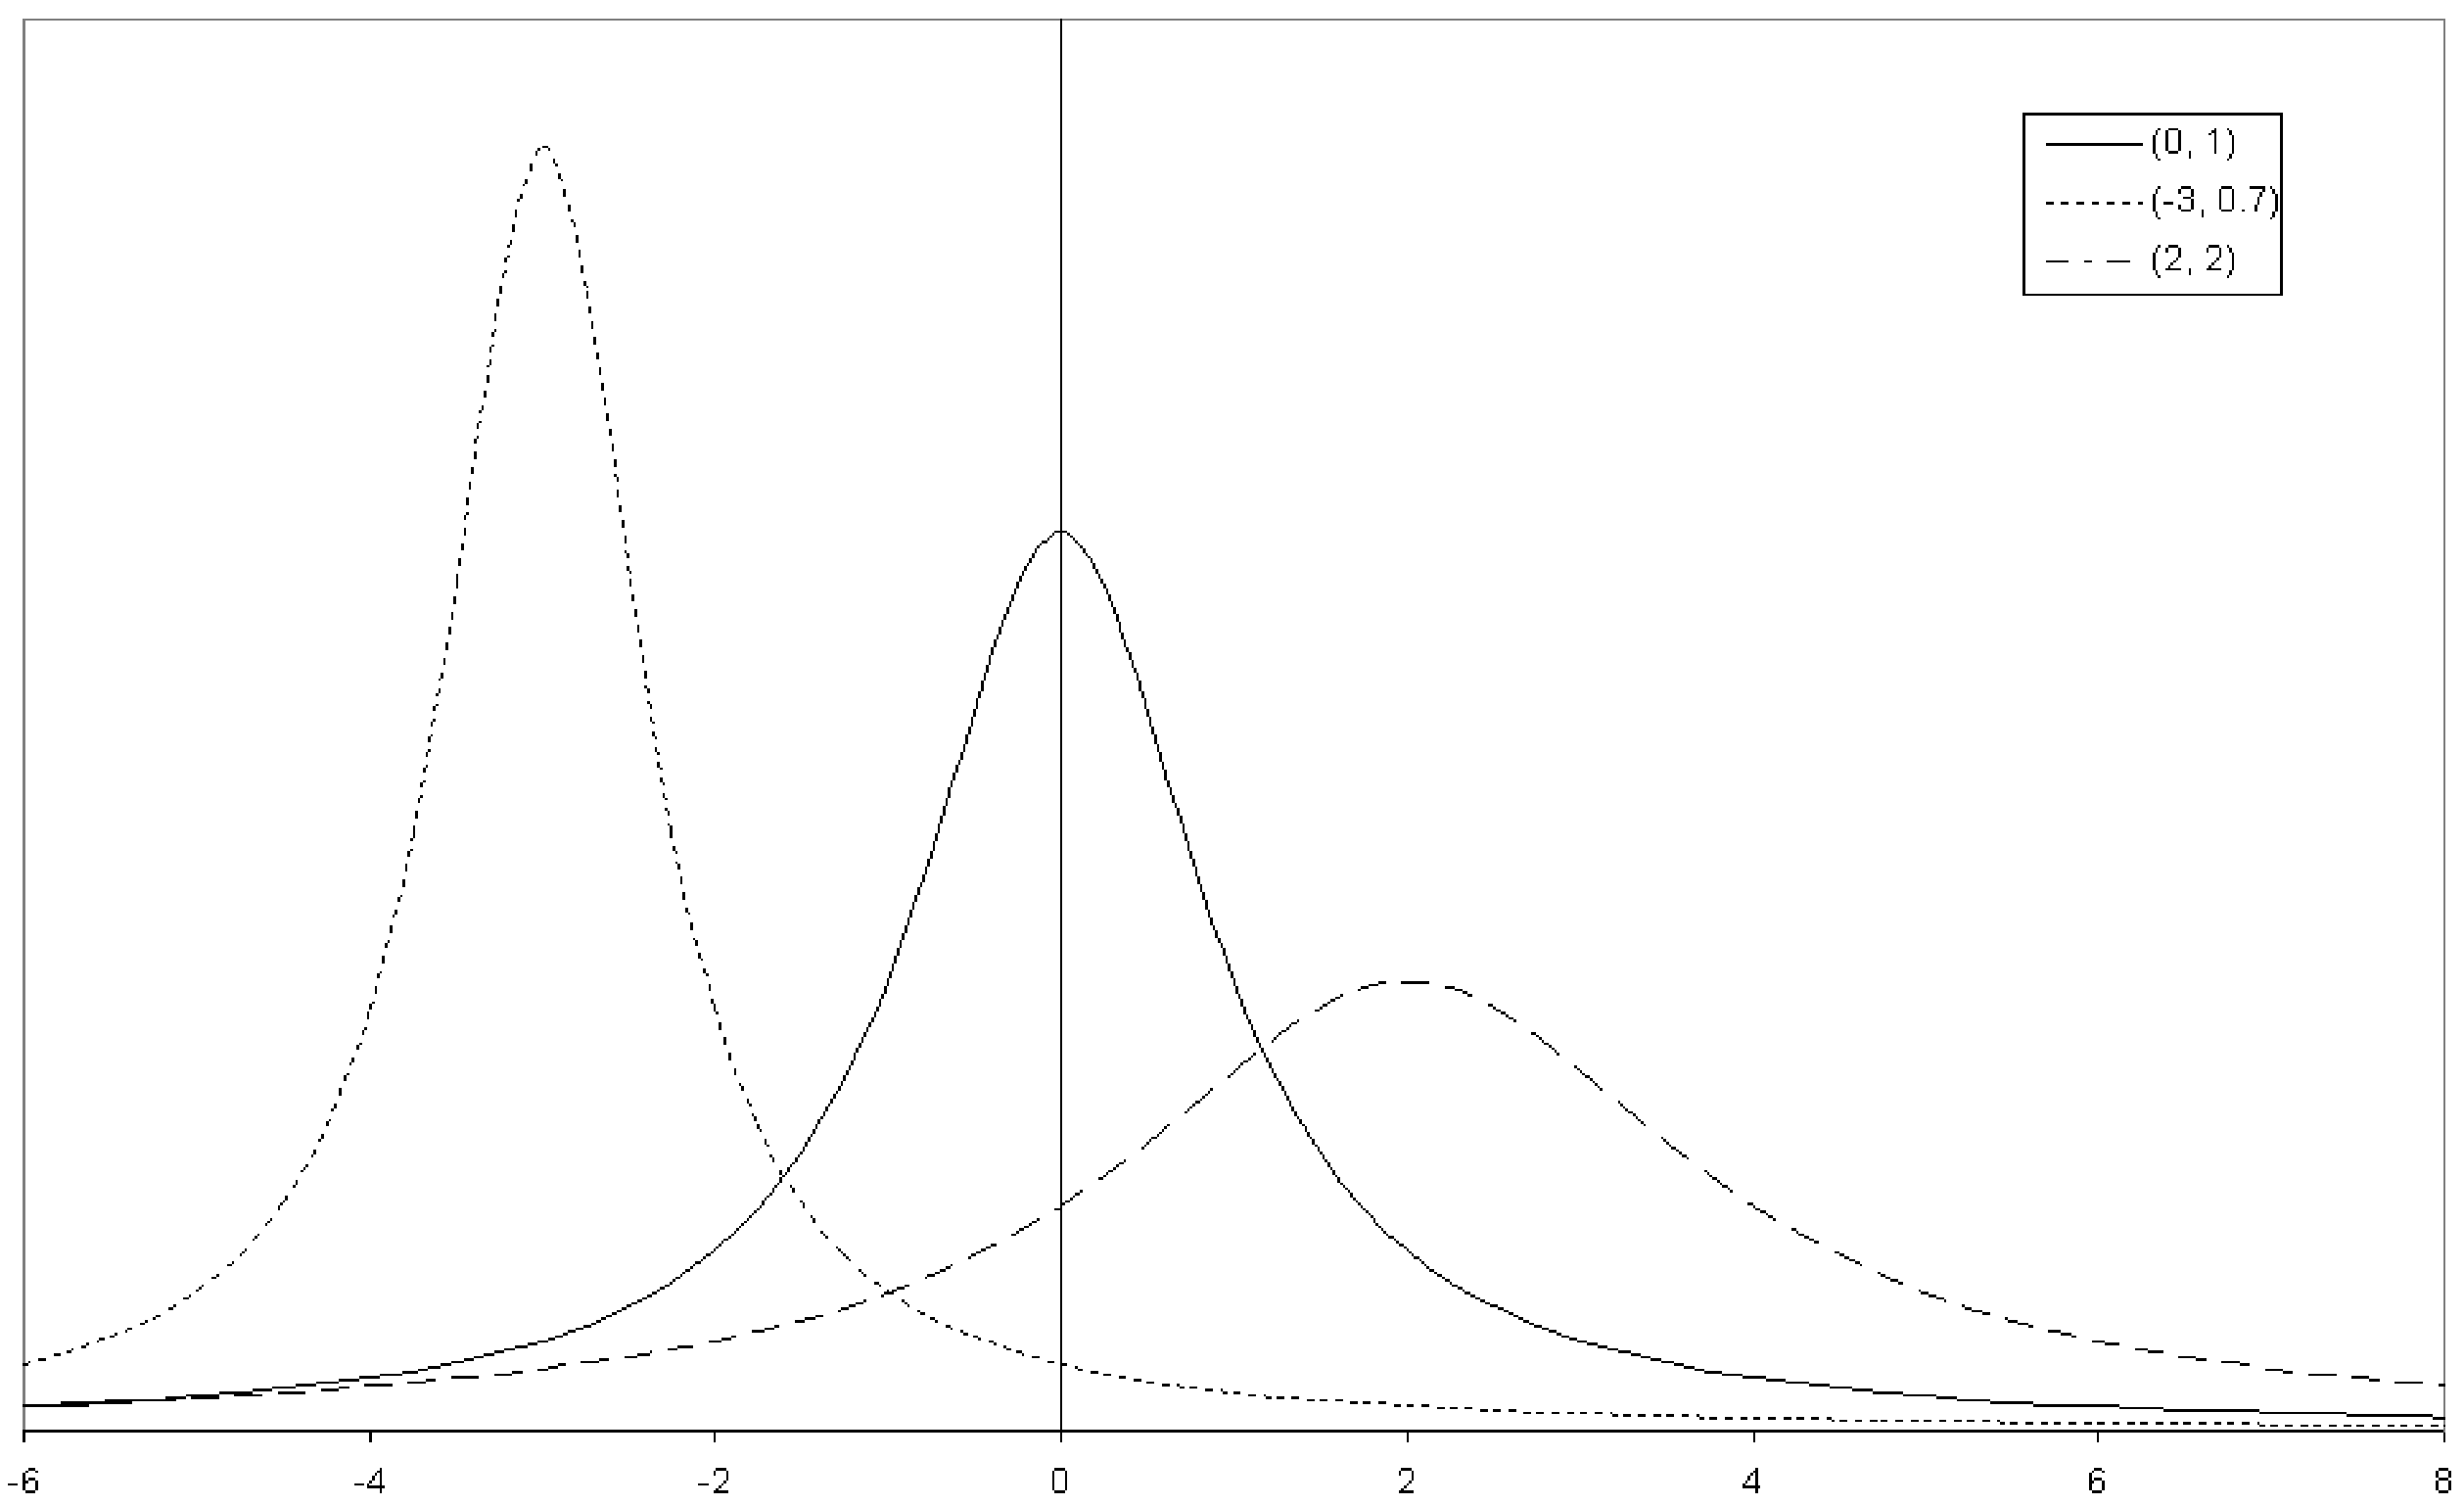
\includegraphics[width=12cm]{Figures/CauchyDistribution}
\caption{Cauchy distribution for a few
parameters}\label{fig:cauchyDistr}
\end{figure}

\subsection{Cauchy distribution --- Smalltalk  implementation}
Listing \ref{ls:cauchydist} shows the implementation of the Cauchy
distribution in Smalltalk.

This implementation returns $\mu$ for the average although the
average is not defined mathematically. Other moment related
quantities are returning {\tt nil}.

\begin{listing} Smalltalk implementation of the Cauchy distribution \label{ls:cauchydist}
$$\halign{ #\hfil&\quad#\hfil\cr {\sl Class}& {\Large\bf DhbCauchyDistribution}\cr
{\sl Subclass of }&{\tt DhbProbabilityDensity}\cr\noalign{\vskip 1ex}

{\sl Instance variable names:}&\parbox[t]{4 in}{\tt  mu beta }\cr\noalign{\vskip 1ex}}$$


Class methods
{\parskip 1ex\par\noindent}
{\bf distributionName}
\begin{verbatim}
    ^'Cauchy distribution'

\end{verbatim}
{\bf fromHistogram:} {\tt aHistogram}
\begin{verbatim}
    ^self shape: aHistogram average
        scale: 4 * aHistogram variance 
                / (Float pi * (aHistogram maximum squared + 
                                         aHistogram minimum squared)) 
                        sqrt

\end{verbatim}
{\bf new}
\begin{verbatim}
    ^self shape: 0 scale: 1

\end{verbatim}
{\bf shape:} {\tt aNumber1} {\bf scale:} {\tt aNumber2}
\begin{verbatim}
    ^super new initialize: aNumber1 scale: aNumber2

\end{verbatim}



Instance methods
{\parskip 1ex\par\noindent}
{\bf acceptanceBetween:} {\tt aNumber1} {\bf and:} {\tt aNumber2}
\begin{verbatim}
    ^self privateAcceptanceBetween: aNumber1 and: aNumber2

\end{verbatim}
{\bf average}
\begin{verbatim}
    ^mu

\end{verbatim}
{\bf changeParametersBy:} {\tt aVector}
\begin{verbatim}
    mu := mu + ( aVector at: 1).
    beta := beta + ( aVector at: 2).

\end{verbatim}
{\bf distributionValue:} {\tt aNumber}
\begin{verbatim}
    ^(( aNumber - mu) / beta) arcTan / Float pi + (1 / 2)

\end{verbatim}
{\bf initialize:} {\tt aNumber1} {\bf scale:} {\tt aNumber2}
\begin{verbatim}
    mu := aNumber1.
    beta := aNumber2.
    ^self

\end{verbatim}
{\bf parameters}
\begin{verbatim}
    ^Array with: mu with: beta

\end{verbatim}
{\bf privateInverseDistributionValue:} {\tt aNumber}
\begin{verbatim}
    ^( ( aNumber - (1 / 2)) * Float pi) tan * beta + mu

\end{verbatim}
{\bf standardDeviation}
\begin{verbatim}
    ^nil

\end{verbatim}
{\bf value:} {\tt aNumber}
\begin{verbatim}
    ^beta / ( Float pi * ( beta squared + ( aNumber - mu) squared))

\end{verbatim}
{\bf valueAndGradient:} {\tt aNumber}
\begin{verbatim}
    | dp denominator |
    dp := self value: aNumber.
    denominator := 1 / ( ( aNumber - mu) squared + beta squared).
    ^Array with: dp
           with: ( DhbVector with: 2 * dp * ( aNumber - mu) * 
                                                           denominator
                             with: dp * ( 1 / beta - ( 2 * beta * 
                                                        denominator)))

\end{verbatim}
{\bf variance}
\begin{verbatim}
    ^nil

\end{verbatim}


\end{listing}


\section{Exponential distribution}
Table \ref{tb:exponentialdist} shows the properties of the
exponential distribution.
\begin{table}[h]
  \centering
  \caption{Properties of the exponential distribution}\label{tb:exponentialdist}
\vspace{1 ex}
\begin{tabular}{|l|c|} \hline
  \vbox to 3ex{}Range of random variable & $\left[0,+\infty\right[$\\ *[1ex] \hline
  \vbox to 4ex{}Probability density function & $\displaystyle P\left(x\right)={1\over\beta}
  e^{-{x\over\beta}}$ \\*[2ex]  \hline
  \vbox to 3ex{}Parameters & $0<\beta<+\infty$ \\*[1ex]  \hline
  \vbox to 4ex{}Distribution function & $\displaystyle F\left(x\right)=1-e^{-{x\over\beta}}$ \\*[1ex]  \hline
  \vbox to 3ex{}Average & $\beta$ \\*[1ex] \hline
  \vbox to 3ex{}Variance & $\beta^2$ \\*[1ex] \hline
  \vbox to 3ex{}Skewness & $2$ \\*[1ex] \hline
  \vbox to 3ex{}Kurtosis & $6$ \\*[1ex] \hline
\end{tabular}
\end{table}

The exponential distribution describes the distribution of the
time of occurrence between independent random events with a
constant probability of occurrence. It is used in queuing theory
and in nuclear physics. Figure \ref{fig:expDistr} shows the shapes
taken by the exponential distribution for a few values of the
parameters.
\begin{figure}
\centering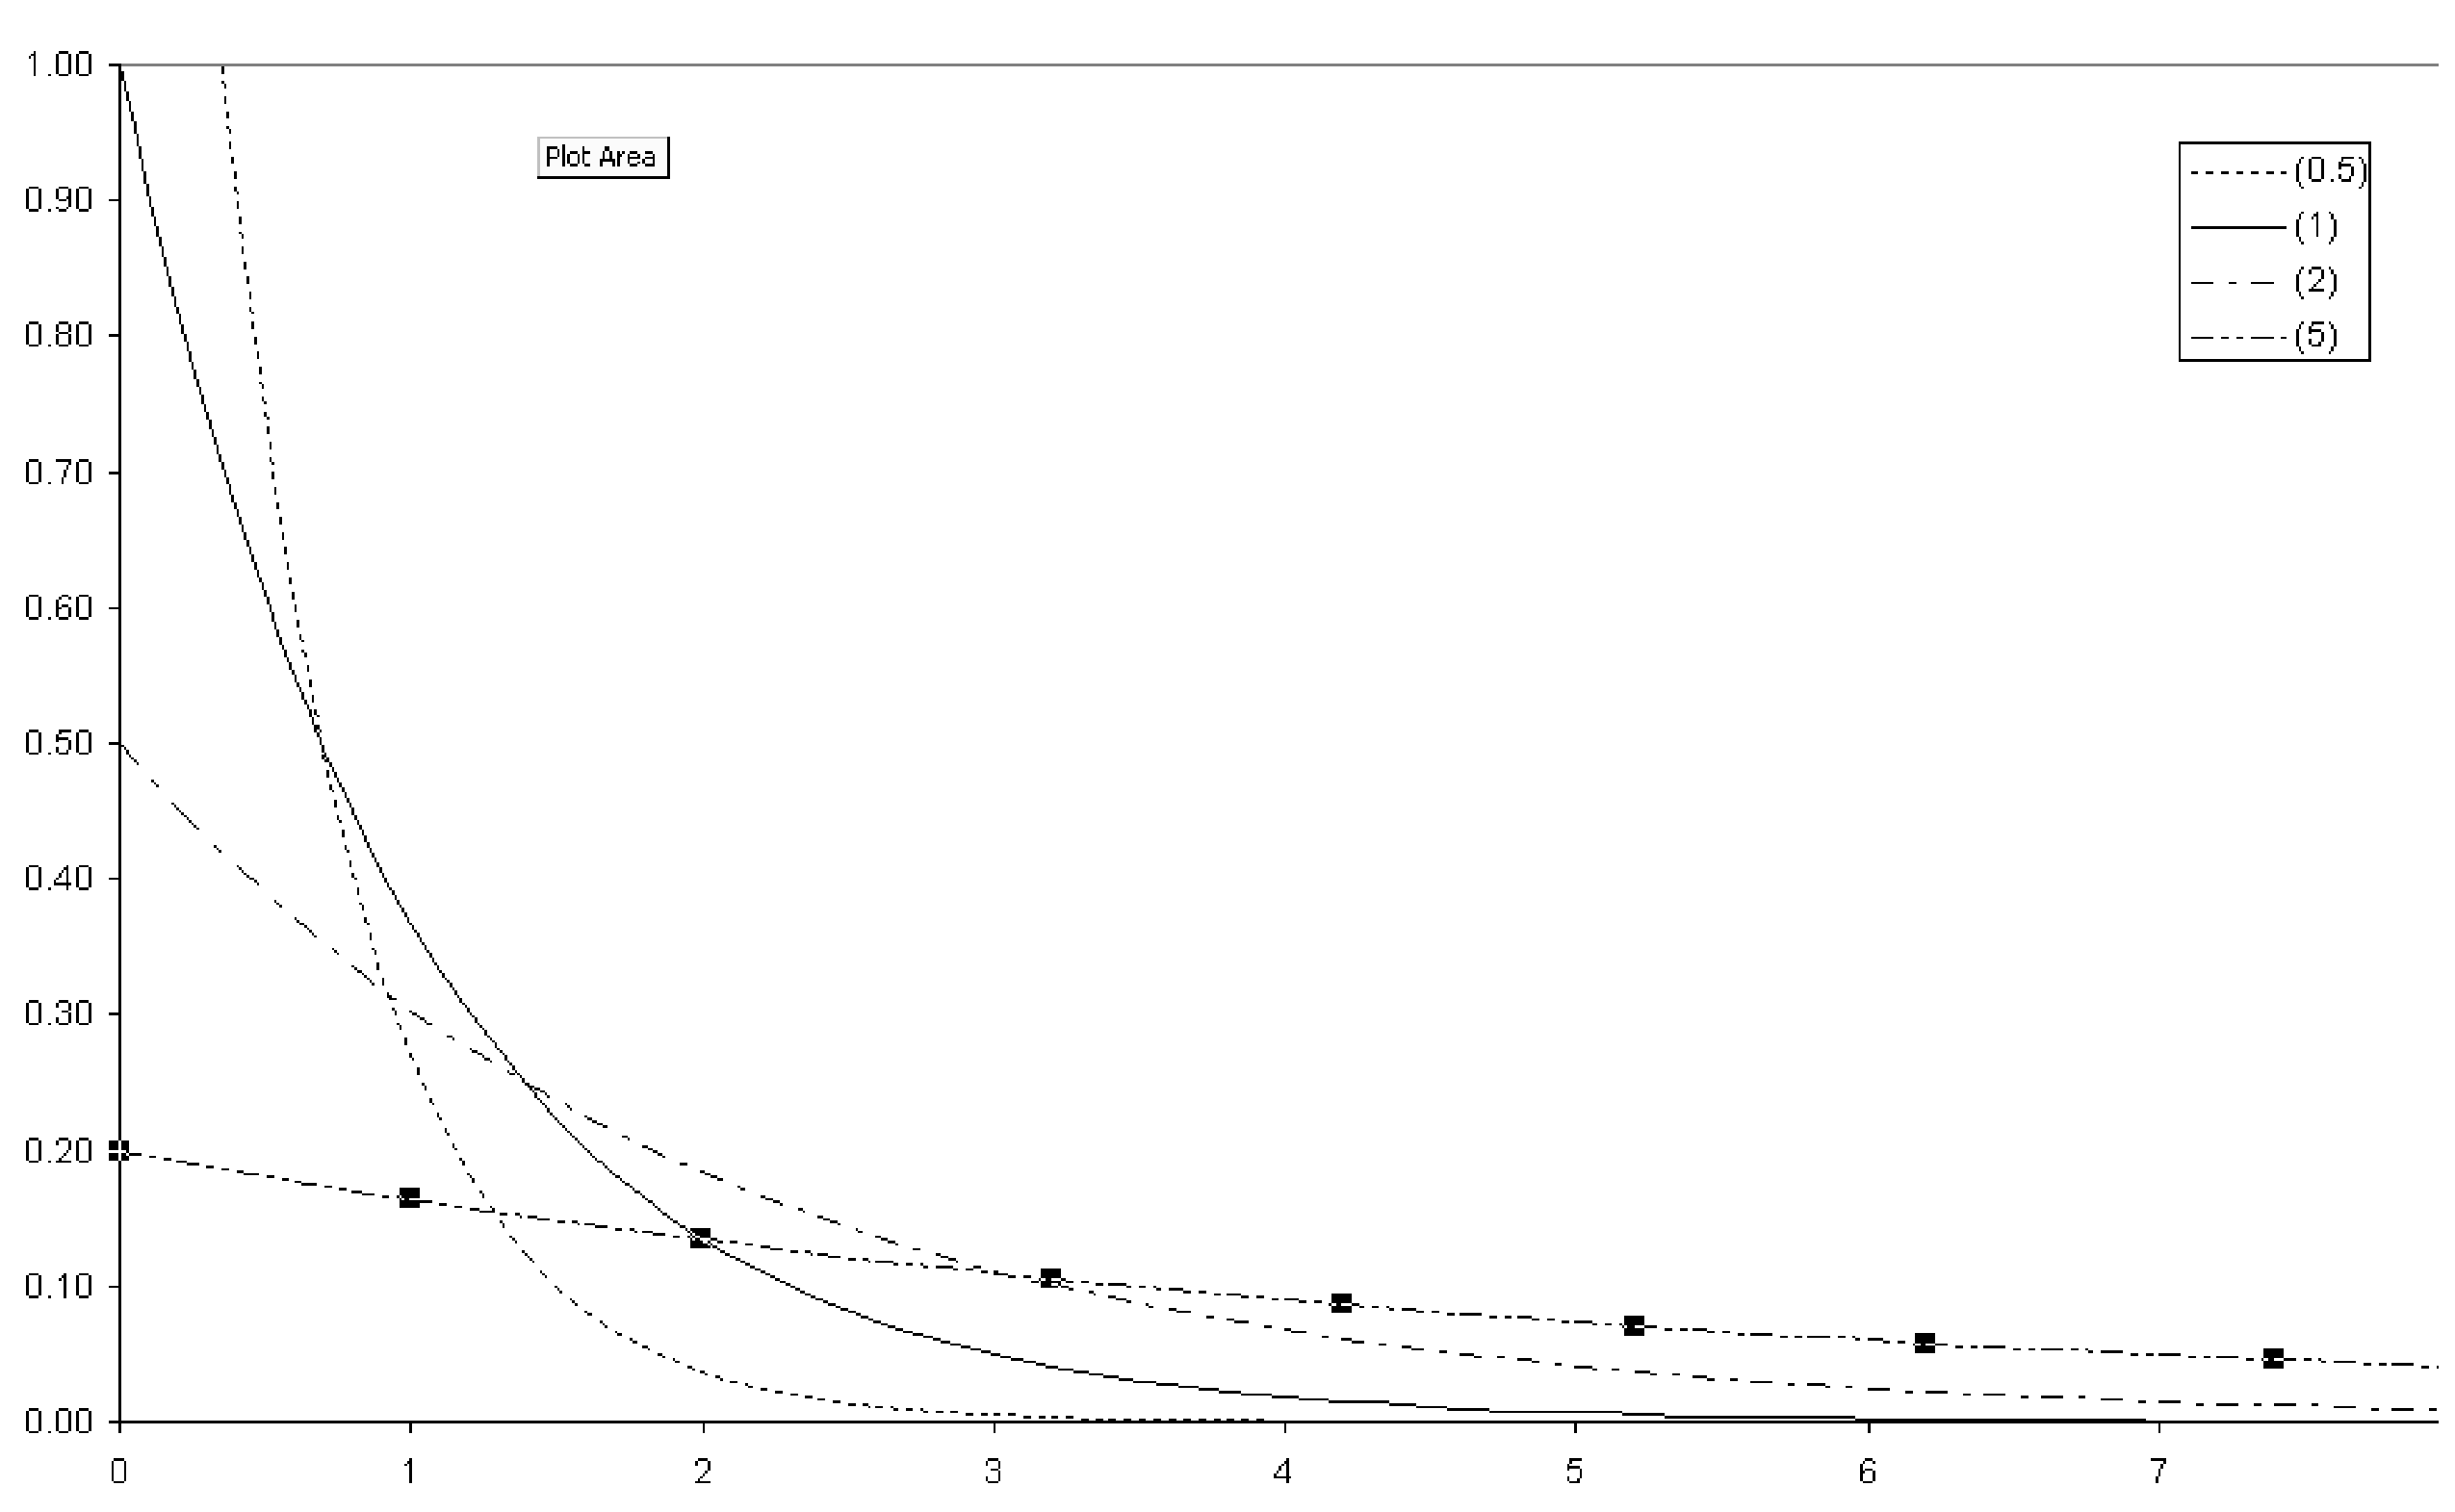
\includegraphics[width=12cm]{Figures/ExponentialDistribution}
\caption{Exponential distribution for a few
parameters}\label{fig:expDistr}
\end{figure}

\subsection{Exponential distribution --- Smalltalk  implementation}
Listing \ref{ls:exponentialdist} shows the implementation of the
exponential distribution in Smalltalk.

\begin{listing} Smalltalk implementation of the exponential distribution \label{ls:exponentialdist}
$$\halign{ #\hfil&\quad#\hfil\cr {\sl Class}& {\Large\bf DhbExponentialDistribution}\cr
{\sl Subclass of }&{\tt DhbProbabilityDensity}\cr\noalign{\vskip 1ex}

{\sl Instance variable names:}&\parbox[t]{4 in}{\tt  beta }\cr\noalign{\vskip 1ex}}$$


Class methods
{\parskip 1ex\par\noindent}
{\bf distributionName}
\begin{verbatim}
    ^'Exponential distribution'

\end{verbatim}
{\bf fromHistogram:} {\tt aHistogram}
\begin{verbatim}
    | mu |
    aHistogram minimum < 0
        ifTrue: [ ^nil].
    mu := aHistogram average.
    ^mu > 0 ifTrue: [ self scale: aHistogram average]
            ifFalse:[ nil]

\end{verbatim}
{\bf new}
\begin{verbatim}
    ^super new initialize: 1

\end{verbatim}
{\bf scale:} {\tt aNumber}
\begin{verbatim}
    ^super new initialize: aNumber

\end{verbatim}



Instance methods
{\parskip 1ex\par\noindent}
{\bf acceptanceBetween:} {\tt aNumber1} {\bf and:} {\tt aNumber2}
\begin{verbatim}
    ^self privateAcceptanceBetween: aNumber1 and: aNumber2

\end{verbatim}
{\bf average}
\begin{verbatim}
    ^beta

\end{verbatim}
{\bf changeParametersBy:} {\tt aVector}
\begin{verbatim}
    beta := beta + ( aVector at: 1).

\end{verbatim}
{\bf distributionValue:} {\tt aNumber}
\begin{verbatim}
    ^[1 - ( ( aNumber / beta negated) exp)]
            when: ExAll do: [ :signal | signal exitWith: 0]

\end{verbatim}
{\bf initialize:} {\tt aNumber}
\begin{verbatim}
    aNumber > 0
        ifFalse: [ self error: 'Illegal distribution parameters'].
    beta := aNumber.
    ^self

\end{verbatim}
{\bf kurtosis}
\begin{verbatim}
    ^6

\end{verbatim}
{\bf parameters}
\begin{verbatim}
    ^Array with: beta

\end{verbatim}
{\bf privateInverseDistributionValue:} {\tt aNumber}
\begin{verbatim}
    ^(1 - aNumber) ln negated * beta

\end{verbatim}
{\bf random}
\begin{verbatim}
    ^DhbMitchellMooreGenerator new floatValue ln * beta negated

\end{verbatim}
{\bf skewness}
\begin{verbatim}
    ^2

\end{verbatim}
{\bf standardDeviation}
\begin{verbatim}
    ^beta

\end{verbatim}
{\bf value:} {\tt aNumber}
\begin{verbatim}
    ^[ ( aNumber / beta) negated exp / beta]
            when: ExAll do: [ :signal | signal exitWith: 0]

\end{verbatim}
{\bf valueAndGradient:} {\tt aNumber}
\begin{verbatim}
    | dp |
    dp := self value: aNumber.
    ^Array with: dp
           with: ( DhbVector with: ( aNumber / beta - 1) * dp / beta)

\end{verbatim}


\end{listing}


\section{Fisher-Tippett distribution}
\label{sec:fishertippettdist} Table \ref{tb:fishertippettdist}
shows the properties of the fishertippett distribution.
\begin{table}[h]
  \centering
  \caption{Properties of the Fisher-Tippett distribution}\label{tb:fishertippettdist}
\vspace{1 ex}
\begin{tabular}{|l|c|} \hline
  \vbox to 3ex{}Range of random variable & $\left]-\infty,+\infty\right[$\\ *[1ex] \hline
  \vbox to 4ex{}Probability density function & $\displaystyle P\left(x\right)=
  {1\over\beta}e^{-{x-\alpha\over\beta}-e^{-{x-\alpha\over\beta}}}$ \\*[2ex]  \hline
  \vbox to 3ex{}Parameters & $-\infty<\alpha<+\infty$ \\
  & $0<\beta<+\infty$\\*[1ex]  \hline
  \vbox to 4ex{}Distribution function & $\displaystyle F\left(x\right)=e^{-e^{-{x-\alpha\over\beta}}}$ \\*[1ex]  \hline
  \vbox to 3ex{}Average & $\alpha+\gamma\beta$ \\*[1ex] \hline
  \vbox to 4ex{}Variance & $\displaystyle{\pi\beta\over\sqrt{6}}$ \\*[2ex] \hline
  \vbox to 3ex{}Skewness & $1.3$ \\*[1ex] \hline
  \vbox to 3ex{}Kurtosis & $2.4$ \\*[1ex] \hline
\end{tabular}
\end{table}
In this table $\gamma=0.5772156649\ldots$ is the Euler constant.

The Fisher-Tippett distribution describes the distribution of
extreme values. Figure \ref{fig:ftippettDistr} shows the shapes
taken by the Fisher-Tippett distribution for a few values of the
parameters. These parameter are identical to the parameters of the
normal distributions shown in figure \ref{fig:normDistr} so that
the reader can compare them.
\begin{figure}
\centering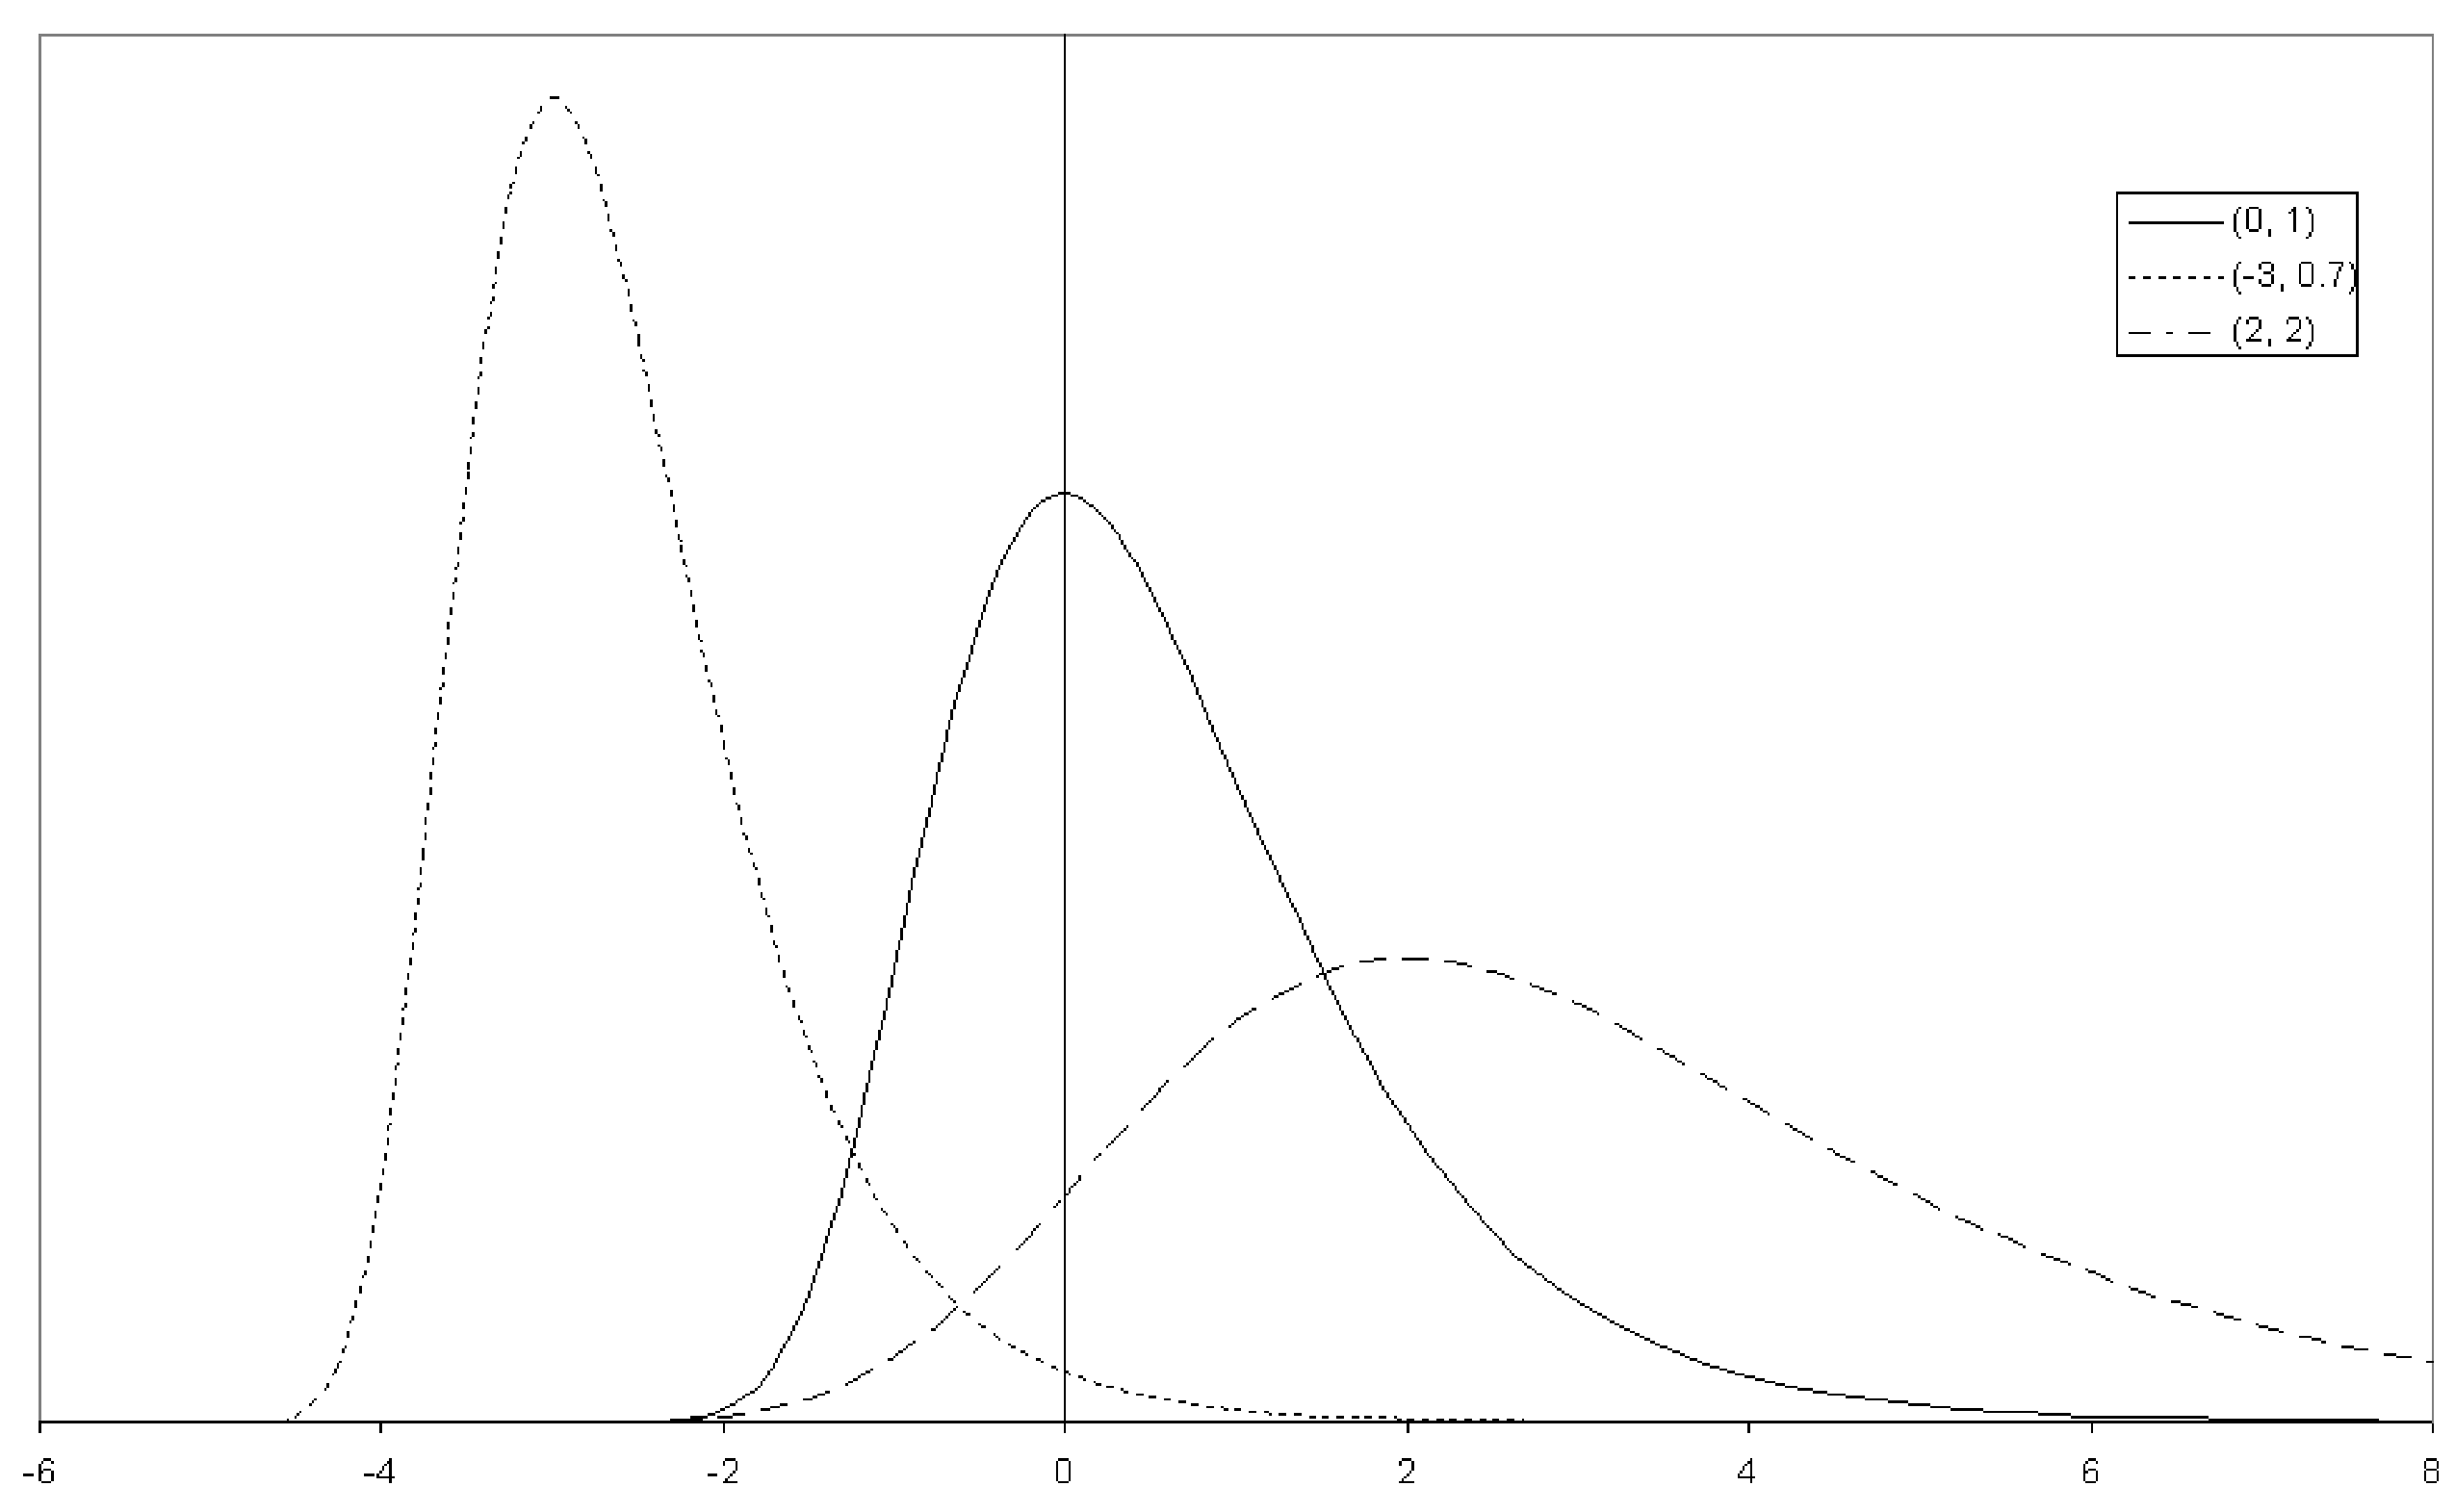
\includegraphics[width=12cm]{Figures/FisherTippettDistribution}
\caption{Fisher-Tippett distribution for a few
parameters}\label{fig:ftippettDistr}
\end{figure}

\subsection{Fisher-Tippett distribution --- Smalltalk  implementation}
Listing \ref{ls:fishertippettdist} shows the implementation of the
Fisher-Tippett distribution in Smalltalk.

\begin{listing} Smalltalk implementation of the Fisher-Tippett distribution \label{ls:fishertippettdist}
$$\halign{ #\hfil&\quad#\hfil\cr {\sl Class}& {\Large\bf DhbFisherTippettDistribution}\cr
{\sl Subclass of }&{\tt DhbProbabilityDensity}\cr\noalign{\vskip 1ex}

{\sl Instance variable names:}&\parbox[t]{4 in}{\tt  alpha beta }\cr\noalign{\vskip 1ex}}$$


Class methods
{\parskip 1ex\par\noindent}
{\bf distributionName}
\begin{verbatim}
    ^'Fisher-Tippett distribution'

\end{verbatim}
{\bf fromHistogram:} {\tt aHistogram}
\begin{verbatim}
    | beta |
    beta := aHistogram standardDeviation.
    beta = 0 ifTrue: [^nil].
    beta := beta * (6 sqrt / Float pi).
    ^self shape: aHistogram average - (0.5772156649 * beta) scale: 
                                                                  beta

\end{verbatim}
{\bf new}
\begin{verbatim}
    ^self shape: 0 scale: 1

\end{verbatim}
{\bf shape:} {\tt aNumber1} {\bf scale:} {\tt aNumber2}
\begin{verbatim}
    ^super new initialize: aNumber1 scale: aNumber2

\end{verbatim}



Instance methods
{\parskip 1ex\par\noindent}
{\bf average}
\begin{verbatim}
    ^0.577256649 * beta + alpha

\end{verbatim}
{\bf changeParametersBy:} {\tt aVector}
\begin{verbatim}
    alpha := alpha + ( aVector at: 1).
    beta := beta + ( aVector at: 2).

\end{verbatim}
{\bf distributionValue:} {\tt aNumber}
\begin{verbatim}
    | arg |
    arg := ( aNumber - alpha) / beta.
    arg := arg < DhbFloatingPointMachine new largestExponentArgument 
                                                               negated
                    ifTrue: [ ^0]
                    ifFalse:[arg negated exp].
    ^arg > DhbFloatingPointMachine new largestExponentArgument 
                                                          ifTrue: [ 1]
                        ifFalse:[ arg negated exp]

\end{verbatim}
{\bf initialize:} {\tt aNumber1} {\bf scale:} {\tt aNumber2}
\begin{verbatim}
    aNumber2 > 0
        ifFalse: [ self error: 'Illegal distribution parameters'].
    alpha := aNumber1.
    beta := aNumber2.
    ^self

\end{verbatim}
{\bf integralFrom:} {\tt aNumber1} {\bf to:} {\tt aNumber2}
\begin{verbatim}
    ^( DhbRombergIntegrator new: self from: aNumber1 to: aNumber2) 
                                                              evaluate

\end{verbatim}
{\bf integralUpTo:} {\tt aNumber}
\begin{verbatim}
    ^( DhbRombergIntegrator new:
            [ :x | x = 0 ifTrue: [ 0] ifFalse: [ ( self value: 1 / x) 
                                                        / x squared] ]
            from: 1 / aNumber to: 0) evaluate

\end{verbatim}
{\bf kurtosis}
\begin{verbatim}
    ^2.4

\end{verbatim}
{\bf parameters}
\begin{verbatim}
    ^Array with: alpha with: beta

\end{verbatim}
{\bf random}
\begin{verbatim}
    | t |
    [ t := DhbMitchellMooreGenerator new floatValue ln negated.
      t > 0] whileFalse: [].
    ^t ln negated * beta + alpha

\end{verbatim}
{\bf skewness}
\begin{verbatim}
    ^1.3

\end{verbatim}
{\bf standardDeviation}
\begin{verbatim}
    ^Float pi * beta / ( 6 sqrt)

\end{verbatim}
{\bf value:} {\tt aNumber}
\begin{verbatim}
    | arg |
    arg := ( aNumber - alpha) / beta.
    arg := arg > DhbFloatingPointMachine new largestExponentArgument 
                                                         ifTrue: [ ^0]
                        ifFalse:[arg negated exp + arg].
    ^arg > DhbFloatingPointMachine new largestExponentArgument 
                                                          ifTrue: [ 0]
                        ifFalse:[ arg negated exp / beta]

\end{verbatim}
{\bf valueAndGradient:} {\tt aNumber}
\begin{verbatim}
    | dp dy y|
    dp := self value: aNumber.
    y := ( aNumber - alpha) / beta.
    dy := ( y negated exp - 1).
    ^Array with: dp
           with: ( DhbVector with: dy * dp / beta negated
                             with: dp * ( y * dy + 1) / beta negated)

\end{verbatim}


\end{listing}


\section{Laplace distribution}
\label{sec:laplacedist} Table \ref{tb:laplacedist} shows the
properties of the Laplace distribution.
\begin{table}[h]
  \centering
  \caption{Properties of the Laplace distribution}\label{tb:laplacedist}
\vspace{1 ex}
\begin{tabular}{|l|c|} \hline
  \vbox to 3ex{}Range of random variable & $\left]-\infty,+\infty\right[$\\ *[1ex] \hline
  \vbox to 4ex{}Probability density function & $\displaystyle P\left(x\right)={1\over 2\beta} e^{-{\left|x-\alpha\right|\over\beta}}$ \\*[2ex]  \hline
  \vbox to 3ex{}Parameters & $-\infty<\alpha<+\infty$ \\
  & $0<\beta<+\infty$\\*[1ex]  \hline
  \vbox to 4ex{}Distribution function &
  \parbox{6cm}{$$F\left(x\right)=\left\{
  \begin{array}{ll}
  {1\over 2}e^{-{\alpha-x\over\beta}}&\mbox{\quad for
  $x<\alpha$}\\*[1ex]
  1-{1\over 2}e^{-{x-\alpha\over\beta}}&\mbox{\quad for $x\ge\alpha$}
  \end{array}\right.$$}\\*[1ex]  \hline
  \vbox to 3ex{}Average & $\alpha+\beta$ \\*[1ex] \hline
  \vbox to 3ex{}Variance & $2\beta^2$ \\*[1ex] \hline
  \vbox to 3ex{}Skewness & $0$ \\*[1ex] \hline
  \vbox to 3ex{}Kurtosis & $3$ \\*[1ex] \hline
\end{tabular}
\end{table}
The Laplace distribution is an ad-hoc distribution made of two
exponential distributions, one on each side of the peak. Figure
\ref{fig:laplaceDistr} shows the shapes taken by the Laplace
distribution for a few values of the parameters. These parameter
are identical to the parameters of the normal distributions shown
in figure \ref{fig:normDistr} so that the reader can compare them.
\begin{figure}
\centering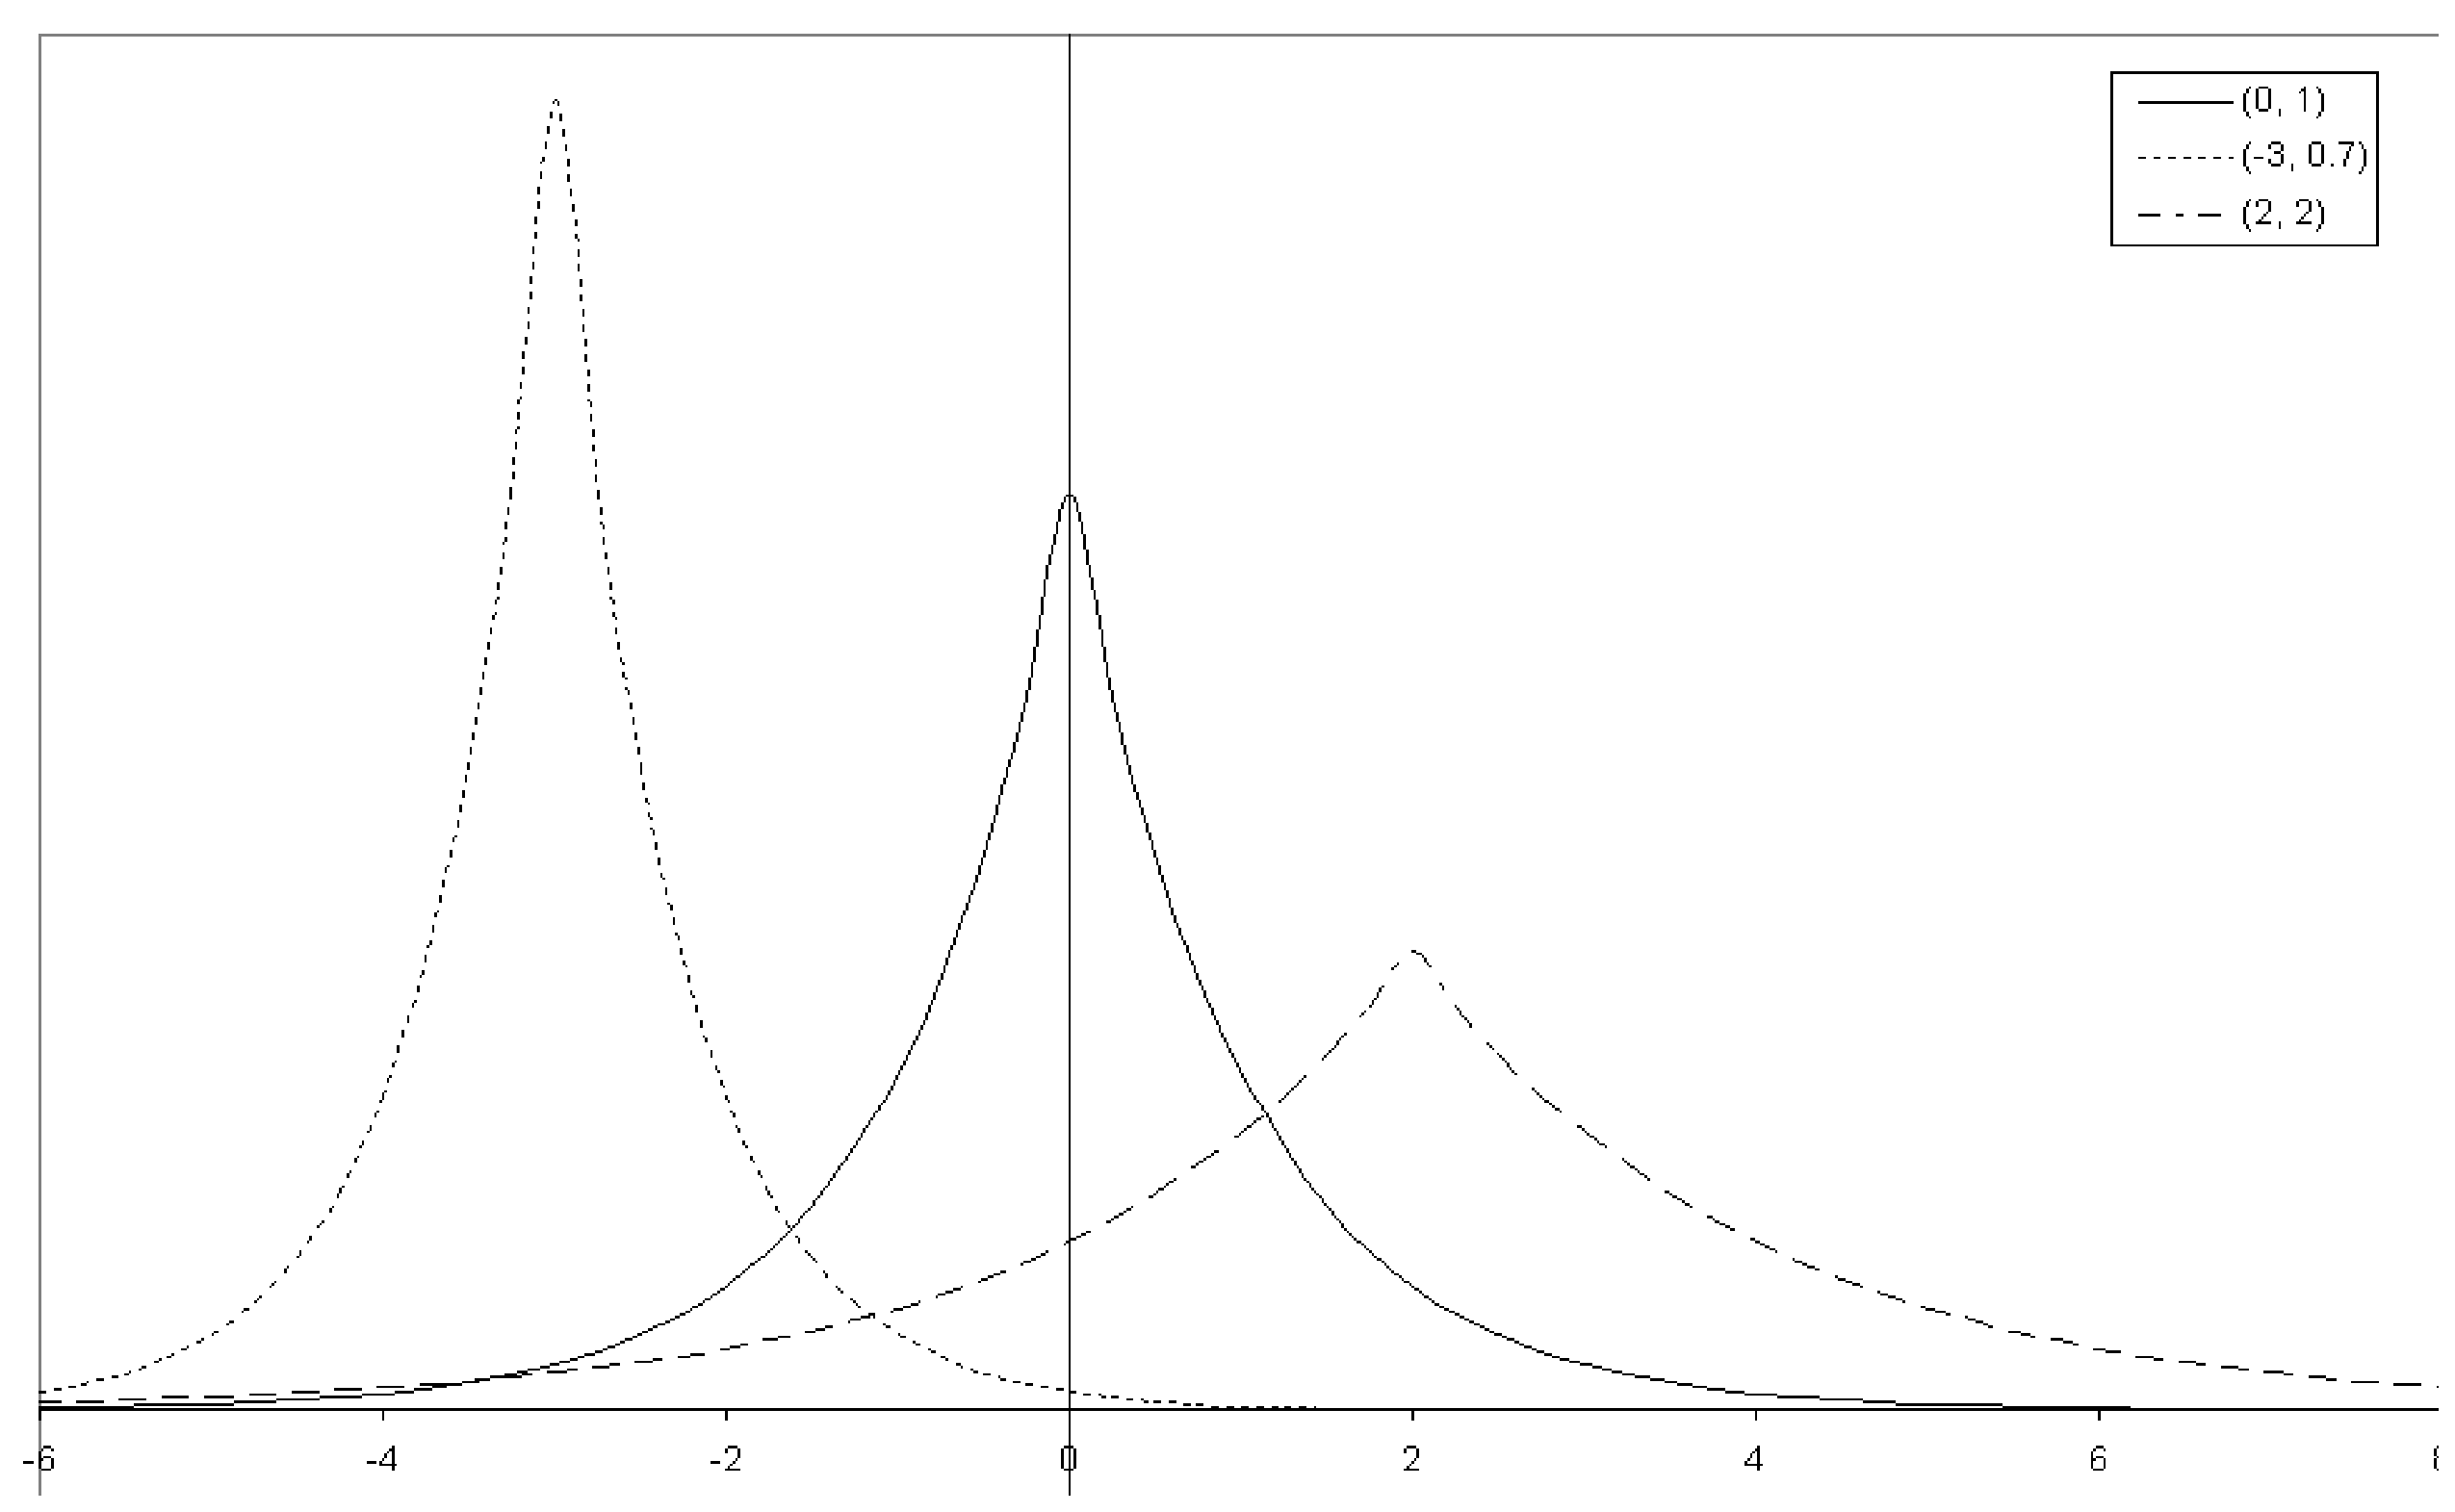
\includegraphics[width=12cm]{Figures/LaplaceDistribution}
\caption{Laplace distribution for a few
parameters}\label{fig:laplaceDistr}
\end{figure}

\subsection{Laplace distribution --- Smalltalk  implementation}
Listing \ref{ls:laplacedist} shows the implementation of the
Laplace distribution in Smalltalk.

\begin{listing} Smalltalk implementation of the Laplace distribution \label{ls:laplacedist}
$$\halign{ #\hfil&\quad#\hfil\cr {\sl Class}& {\Large\bf DhbLaplaceDistribution}\cr
{\sl Subclass of }&{\tt DhbProbabilityDensity}\cr\noalign{\vskip 1ex}

{\sl Instance variable names:}&\parbox[t]{4 in}{\tt  mu beta }\cr\noalign{\vskip 1ex}}$$


Class methods
{\parskip 1ex\par\noindent}
{\bf distributionName}
\begin{verbatim}
    ^'Laplace distribution'

\end{verbatim}
{\bf fromHistogram:} {\tt aHistogram}
\begin{verbatim}
    ^self shape: aHistogram average scale: (aHistogram variance / 2) 
                                                                  sqrt

\end{verbatim}
{\bf new}
\begin{verbatim}
    ^self shape: 0 scale: 1

\end{verbatim}
{\bf shape:} {\tt aNumber1} {\bf scale:} {\tt aNumber2}
\begin{verbatim}
    ^super new initialize: aNumber1 scale: aNumber2

\end{verbatim}



Instance methods
{\parskip 1ex\par\noindent}
{\bf average}
\begin{verbatim}
    ^mu

\end{verbatim}
{\bf changeParametersBy:} {\tt aVector}
\begin{verbatim}
    mu := mu + ( aVector at: 1).
    beta := beta + ( aVector at: 2).

\end{verbatim}
{\bf distributionValue:} {\tt aNumber}
\begin{verbatim}
    ^aNumber > mu
        ifTrue: [ 1 - ( ( ( aNumber - mu) / beta) negated exp / 2)]
        ifFalse:[ ( ( ( aNumber - mu) / beta) exp / 2)]

\end{verbatim}
{\bf initialize:} {\tt aNumber1} {\bf scale:} {\tt aNumber2}
\begin{verbatim}
    mu := aNumber1.
    beta := aNumber2.
    ^self

\end{verbatim}
{\bf kurtosis}
\begin{verbatim}
    ^3

\end{verbatim}
{\bf parameters}
\begin{verbatim}
    ^Array with: mu with: beta

\end{verbatim}
{\bf random}
\begin{verbatim}
    | r |
    r := DhbMitchellMooreGenerator new floatValue ln * beta negated.
    ^DhbMitchellMooreGenerator new floatValue > 0.5
        ifTrue: [ mu + r]
        ifFalse:[ mu - r]

\end{verbatim}
{\bf skewness}
\begin{verbatim}
    ^0

\end{verbatim}
{\bf standardDeviation}
\begin{verbatim}
    ^beta * ( 2 sqrt)

\end{verbatim}
{\bf value:} {\tt aNumber}
\begin{verbatim}
    ^( ( aNumber - mu) / beta) abs negated exp / ( 2 * beta)

\end{verbatim}
{\bf valueAndGradient:} {\tt aNumber}
\begin{verbatim}
    | dp |
    dp := self value: aNumber.
    ^Array  with: dp
            with: ( DhbVector with: ( aNumber - mu) sign * dp / beta
                              with: ( ( ( aNumber - mu) abs / beta - 
                                                      1) * dp / beta))

\end{verbatim}


\end{listing}


\section{Log normal  distribution}
Table \ref{tb:lognormaldist} shows the properties of the log
normal distribution.
\begin{table}[h]
  \centering
  \caption{Properties of the log normal distribution}\label{tb:lognormaldist}
\vspace{1 ex}
\begin{tabular}{|l|c|} \hline
  \vbox to 3ex{}Range of random variable & $\left[0,+\infty\right[$\\ *[1ex] \hline
  \vbox to 4ex{}Probability density function & $\displaystyle P\left(x\right)=
  {1\over x\sqrt{2\pi\sigma^2}}e^{-{\left(\ln x-\mu\right)^2\over 2\sigma^2}}$ \\*[2ex]  \hline
  \vbox to 3ex{}Parameters & $-\infty<\mu<+\infty$ \\
  & $0<\sigma<+\infty$\\*[1ex]  \hline
  \vbox to 4ex{}Distribution function & (no closed expression) \\*[1ex]  \hline
  \vbox to 3ex{}Average & $e^{\mu+{\sigma^2\over 2}}$ \\*[1ex] \hline
  \vbox to 4ex{}Variance & $e^{2\mu+\sigma^2}\left(e^{\sigma^2}-1\right)$ \\*[1ex] \hline
  \vbox to 4ex{}Skewness & $\sqrt{e^{\sigma^2}-1}\left(e^{\sigma^2}+2\right)$ \\*[2ex] \hline
  \vbox to 3ex{}Kurtosis & $ e^{4\sigma^2}+2e^{3\sigma^2}+3e^{2\sigma^2}-6$ \\*[1ex] \hline
\end{tabular}
\end{table}
The log normal distribution is used to describe quantities that
are the product of a large number of other quantities. It is an
ad-hoc distribution whose shape is similar to that of gamma
distributions with $\alpha>1$. Figure \ref{fig:logNormDistr} shows
the shapes taken by the log normal distribution for a few values
of the parameters.
\begin{figure}
\centering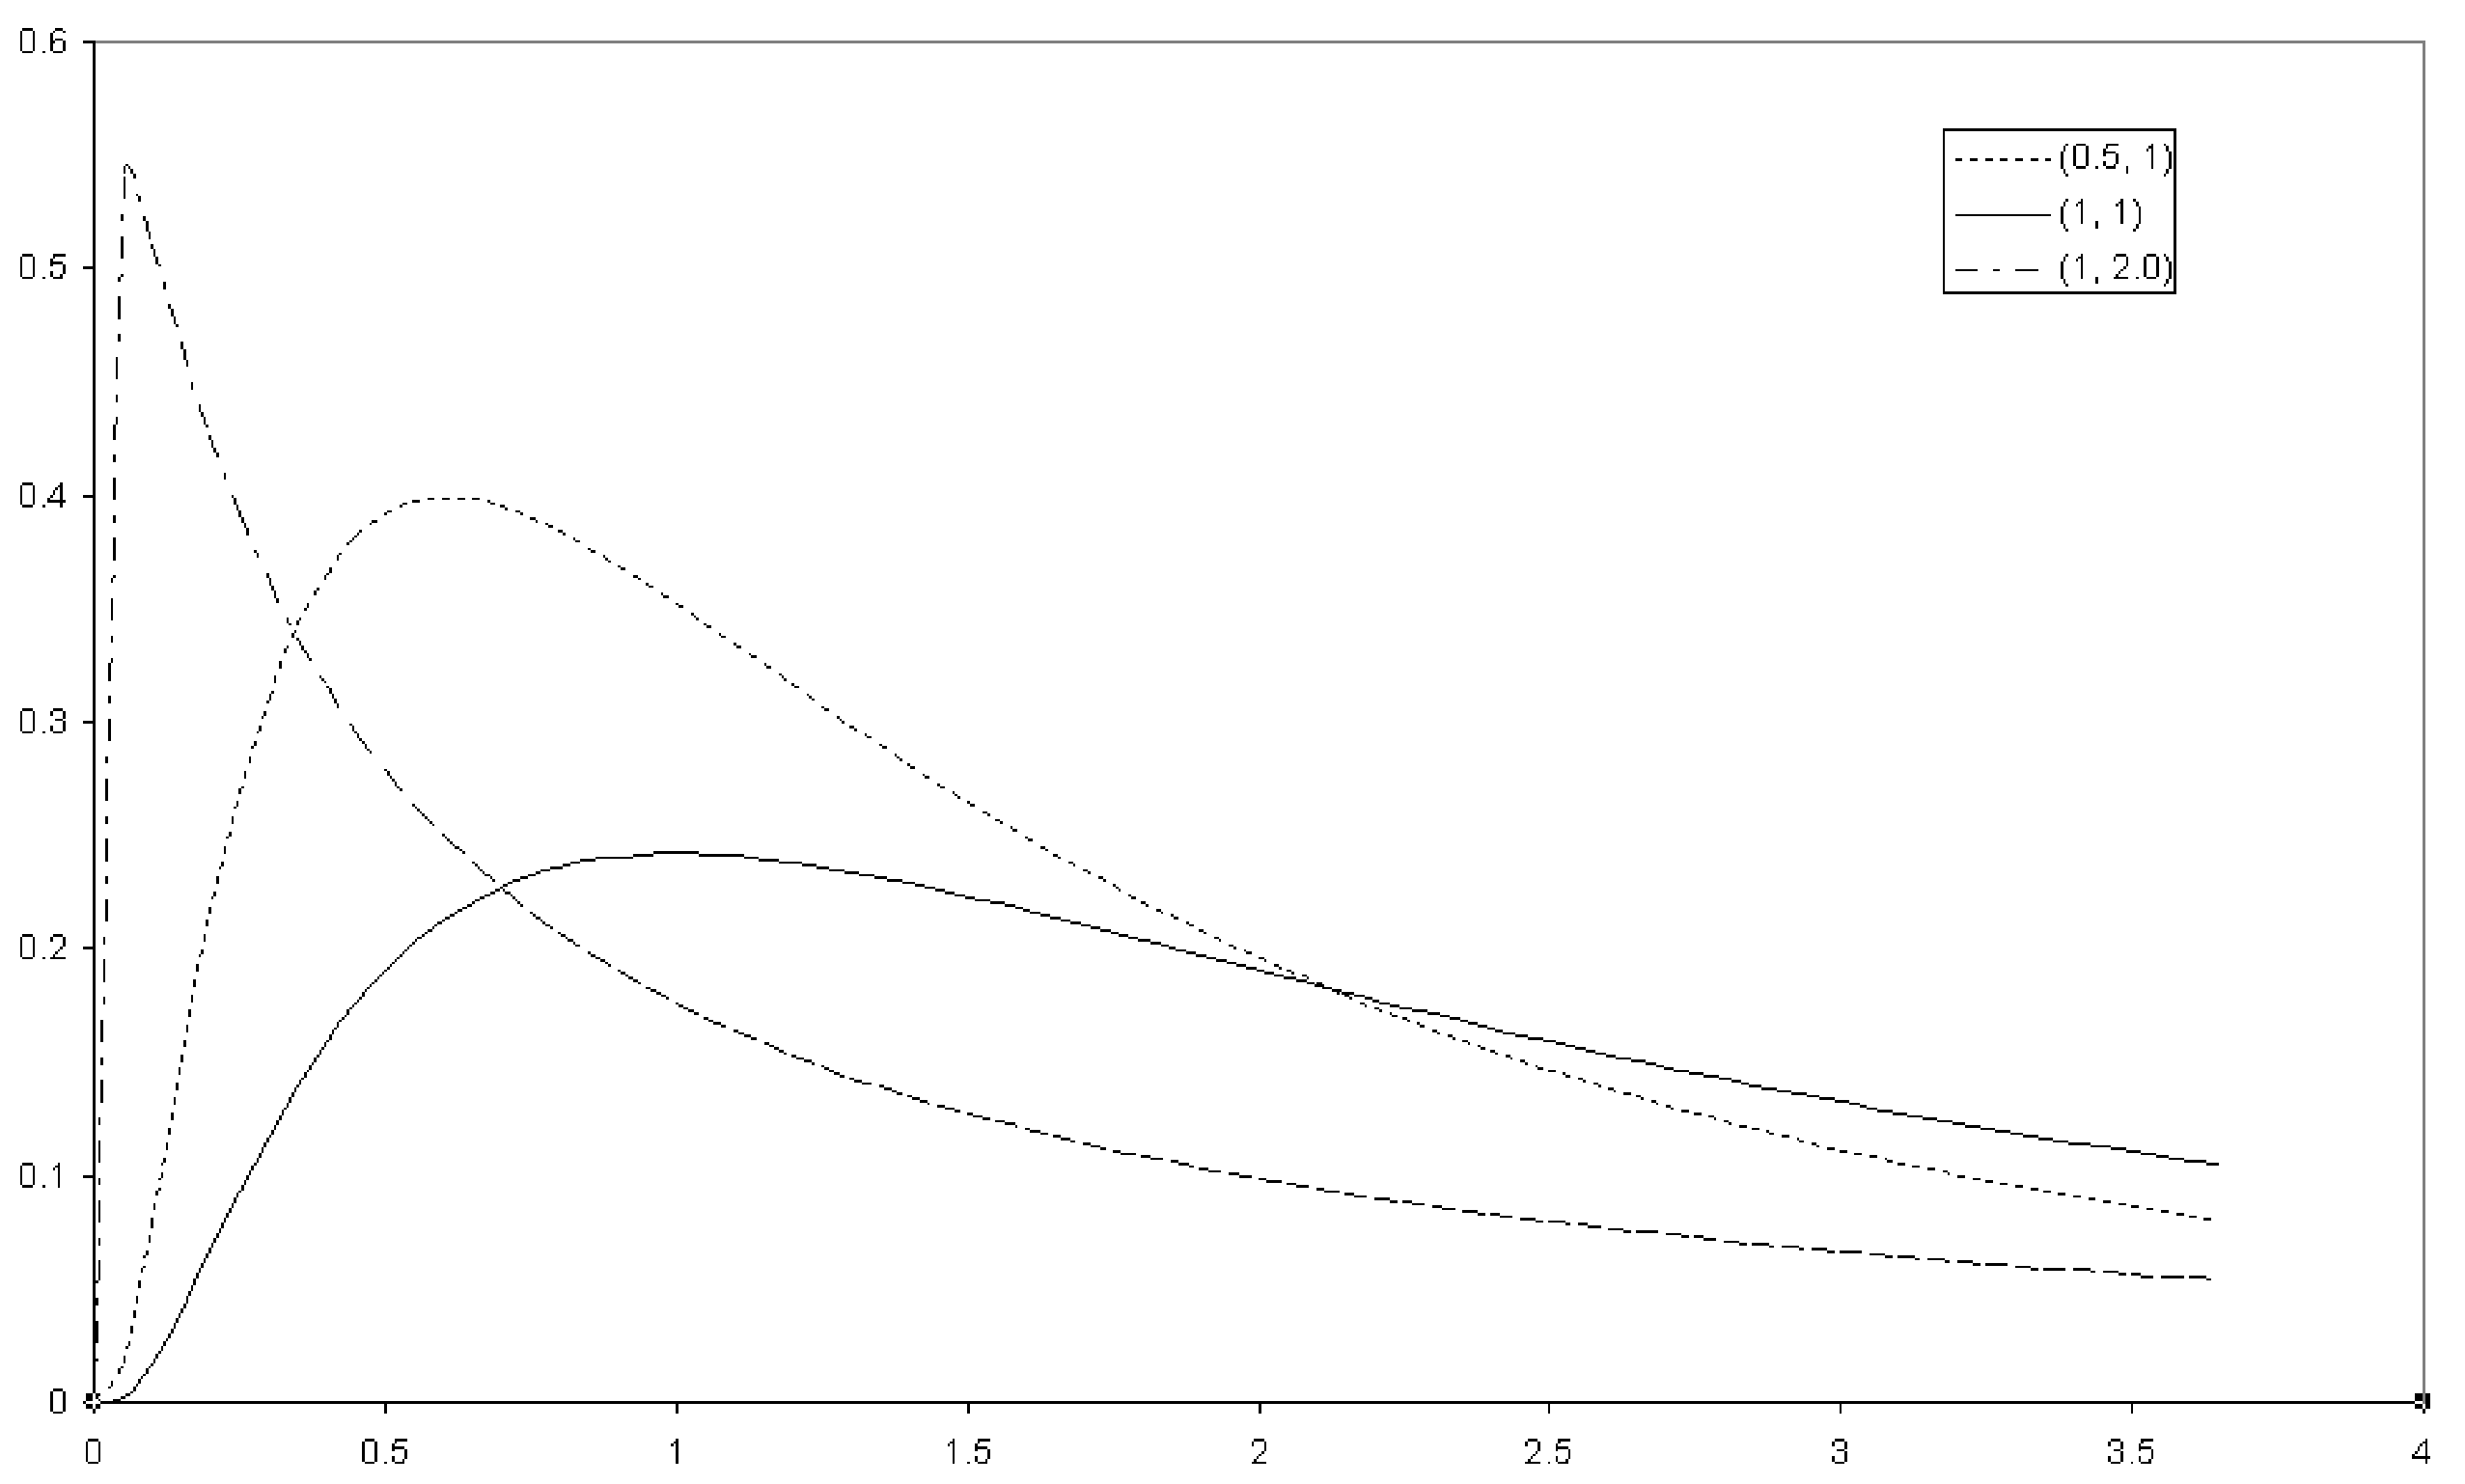
\includegraphics[width=12cm]{Figures/LogNormalDistribution}
\caption{Log normal distribution for a few parameters}\label{fig:logNormDistr}
\end{figure}

\subsection{Log normal distribution --- Smalltalk  implementation}
Listing \ref{ls:lognormaldist} shows the implementation of the log
normal  distribution in Smalltalk.

\begin{listing} Smalltalk implementation of the log normal distribution \label{ls:lognormaldist}
$$\halign{ #\hfil&\quad#\hfil\cr {\sl Class}& {\Large\bf DhbLogNormalDistribution}\cr
{\sl Subclass of }&{\tt DhbProbabilityDensityWithUnknownDistribution}\cr\noalign{\vskip 1ex}

{\sl Instance variable names:}&\parbox[t]{4 in}{\tt  normalDistribution }\cr\noalign{\vskip 1ex}}$$


Class methods
{\parskip 1ex\par\noindent}
{\bf distributionName}
\begin{verbatim}
    ^'Log normal distribution'

\end{verbatim}
{\bf fromHistogram:} {\tt aHistogram}
\begin{verbatim}
    | average variance sigma2 |
    aHistogram minimum < 0
        ifTrue: [ ^nil].
    average := aHistogram average.
    average > 0
        ifFalse: [ ^nil].
    variance := aHistogram variance.
    sigma2 := ( variance / average squared + 1) ln.
    sigma2 > 0
        ifFalse: [ ^nil].
    ^self new: ( average ln - (sigma2 * 0.5)) sigma: sigma2 sqrt

\end{verbatim}
{\bf new}
\begin{verbatim}
    ^self new: 0 sigma: 1

\end{verbatim}
{\bf new:} {\tt aNumber1} {\bf sigma:} {\tt aNumber2}
\begin{verbatim}
    ^super new initialize: aNumber1 sigma: aNumber2

\end{verbatim}



Instance methods
{\parskip 1ex\par\noindent}
{\bf average}
\begin{verbatim}
    ^( normalDistribution variance * 0.5 + normalDistribution 
                                                          average) exp

\end{verbatim}
{\bf changeParametersBy:} {\tt aVector}
\begin{verbatim}
    normalDistribution changeParametersBy: aVector.

\end{verbatim}
{\bf fourthCentralMoment}
\begin{verbatim}
    | y x |
    y := normalDistribution average exp.
    x := normalDistribution variance exp.
    ^( y squared squared) * ( x squared)
        * ( ( ( x squared * x - 4) * ( x squared) + 6) * x - 3)

\end{verbatim}
{\bf initialize:} {\tt aNumber1} {\bf sigma:} {\tt aNumber2}
\begin{verbatim}
    normalDistribution := DhbNormalDistribution new: aNumber1 sigma: 
                                                             aNumber2.
    ^self

\end{verbatim}
{\bf kurtosis}
\begin{verbatim}
    | x |
    x := normalDistribution variance exp.
    ^( ( x + 2) * x + 3) * ( x squared) - 6

\end{verbatim}
{\bf parameters}
\begin{verbatim}
    ^normalDistribution parameters

\end{verbatim}
{\bf random}
\begin{verbatim}
    ^normalDistribution random exp

\end{verbatim}
{\bf skewness}
\begin{verbatim}
    | x |
    x := normalDistribution variance exp.
    ^(x - 1) sqrt * (x + 2)

\end{verbatim}
{\bf thirdCentralMoment}
\begin{verbatim}
    | y x |
    y := normalDistribution average exp.
    x := normalDistribution variance exp.
    ^( y squared * y) * ( x raisedTo: (3/2))
        * ( ( x squared negated + 3) * x - 2)

\end{verbatim}
{\bf value:} {\tt aNumber}
\begin{verbatim}
    ^aNumber > 0
        ifTrue: [ ( normalDistribution value: aNumber ln) / aNumber]
        ifFalse:[ 0]

\end{verbatim}
{\bf variance}
\begin{verbatim}
    ^( normalDistribution average * 2 + normalDistribution variance) 
                          exp * ( normalDistribution variance exp - 1)

\end{verbatim}


\end{listing}


\section{Triangular distribution}
Table \ref{tb:triangdist} shows the properties of the triangular
distribution.
\begin{table}[h]
  \centering
  \caption{Properties of the triangular distribution}\label{tb:triangdist}
\vspace{1 ex}
\begin{tabular}{|l|c|} \hline
  \vbox to 3ex{}Range of random variable & $\left[a,b\right]$\\ *[1ex] \hline
  \vbox to 4ex{}Probability density function & \parbox{6cm}{$$\displaystyle P\left(x\right)=
  \left\{\begin{array}{ll}
  {2\left(x-a\right)\over\left(b-a\right)\left(c-a\right)}&\mbox{\quad if $a\le x\le
  c$,}\\*[3ex]
  {2\left(b-x\right)\over\left(b-a\right)\left(b-c\right)}&\mbox{\quad if $c\le x\le
  b$.}
  \end{array}
  \right.$$} \\*[2ex]  \hline
  \vbox to 3ex{}Parameters & $-\infty<a\le c\le b<+\infty$ \\
  & $a<b$\\*[1ex]  \hline
  \vbox to 4ex{}Distribution function & \parbox{8cm}{$$\displaystyle F\left(x\right)=
  \left\{\begin{array}{ll}
  {\left(x-a\right)^2\over\left(b-a\right)\left(c-a\right)}&\mbox{\quad if $a\le x\le
  c$,}\\*[3ex]
  1-{\left(b-x\right)^2\over\left(b-a\right)\left(b-c\right)}&\mbox{\quad if $c\le x\le
  b$.}
  \end{array}
  \right.$$} \\*[1ex]  \hline
  \vbox to 4ex{}Average & $\displaystyle{a+b+c\over 3}$ \\*[1ex] \hline
  \vbox to 4ex{}Variance & $\displaystyle{a^2+b^2+c^2-ab-ac-bc\over 18}$ \\*[1ex] \hline
  \vbox to 4ex{}Skewness & $\displaystyle{a^3+b^3+c^3\over 135}+\ldots$ \\*[1ex] \hline
  \vbox to 4ex{}Kurtosis & $\ldots$ \\*[1ex] \hline
\end{tabular}
\end{table}
The triangular distribution is ad-hoc distribution used when a
variable is limited to an interval.

\subsection{Triangular distribution --- Smalltalk  implementation}
Listing \ref{ls:triangdist} shows the implementation of the
triangular distribution in Smalltalk.

\begin{listing} Smalltalk implementation of the triangular distribution \label{ls:triangdist}
$$\halign{ #\hfil&\quad#\hfil\cr {\sl Class}& {\Large\bf DhbTriangularDistribution}\cr
{\sl Subclass of }&{\tt DhbProbabilityDensity}\cr\noalign{\vskip 1ex}

{\sl Instance variable names:}&\parbox[t]{4 in}{\tt  lowLimit highLimit peak }\cr\noalign{\vskip 1ex}}$$


Class methods
{\parskip 1ex\par\noindent}
{\bf distributionName}
\begin{verbatim}
    ^'Triangular distribution'

\end{verbatim}
{\bf fromHistogram:} {\tt aHistogram}
\begin{verbatim}
    | b c|
    b := aHistogram standardDeviation * 1.73205080756888 

\end{verbatim}
{\bf new}
\begin{verbatim}
    ^self new: (1 / 2) from: 0 to: 1

\end{verbatim}
{\bf new:} {\tt aNumber1} {\bf from:} {\tt aNumber2} {\bf to:} {\tt aNumber3}
\begin{verbatim}
    ^super new initialize: aNumber1 from: aNumber2 to: aNumber3

\end{verbatim}



Instance methods
{\parskip 1ex\par\noindent}
{\bf acceptanceBetween:} {\tt aNumber1} {\bf and:} {\tt aNumber2}
\begin{verbatim}
    ^self privateAcceptanceBetween: aNumber1 and: aNumber2

\end{verbatim}
{\bf average}
\begin{verbatim}
    ^(lowLimit + peak + highLimit) / 3

\end{verbatim}
{\bf changeParametersBy:} {\tt aVector}
\begin{verbatim}
    lowLimit := lowLimit + ( aVector at: 1).
    highLimit := highLimit + ( aVector at: 2).
    peak := peak + ( aVector at: 3).

\end{verbatim}
{\bf distributionValue:} {\tt aNumber}
\begin{verbatim}
    | norm |
    ^( aNumber between: lowLimit and: highLimit)
        ifTrue: [ aNumber < peak
                        ifTrue: [ norm := ( highLimit - lowLimit) * ( 
                                                     peak - lowLimit).
                                     ( aNumber - lowLimit) squared / 
                                                                  norm
                                    ]
                        ifFalse:[ aNumber > peak
                                        ifTrue: [ norm := ( highLimit 
                                    - lowLimit) * ( highLimit - peak).
                                                     1 - ( ( 
                                  highLimit - aNumber) squared / norm)
                                                    ]
                                        ifFalse:[ ( peak - lowLimit) 
                                            / ( highLimit - lowLimit)]
                                    ]
                   ]
        ifFalse:[ 0]

\end{verbatim}
{\bf initialize:} {\tt aNumber1} {\bf from:} {\tt aNumber2} {\bf to:} {\tt aNumber3}
\begin{verbatim}
    ( aNumber2 < aNumber3 and: [ aNumber1 between: aNumber2 and: 
                                                            aNumber3])
        ifFalse: [ self error: 'Illegal distribution parameters'].
    peak := aNumber1.
    lowLimit := aNumber2.
    highLimit := aNumber3.
    ^self

\end{verbatim}
{\bf inverseAcceptanceAfterPeak:} {\tt aNumber}
\begin{verbatim}
    ^ highLimit - ( ( ( 1 - aNumber) * ( highLimit - lowLimit) * ( 
                                              highLimit - peak)) sqrt)

\end{verbatim}
{\bf inverseAcceptanceBeforePeak:} {\tt aNumber}
\begin{verbatim}
    ^ ( aNumber * ( highLimit - lowLimit) * ( peak - lowLimit)) sqrt 
                                                            + lowLimit

\end{verbatim}
{\bf kurtosis}
\begin{verbatim}
    ^(-6/10)

\end{verbatim}
{\bf parameters}
\begin{verbatim}
    ^Array with: lowLimit with: highLimit with: peak

\end{verbatim}
{\bf privateInverseDistributionValue:} {\tt aNumber}
\begin{verbatim}
    ^( peak - lowLimit) / ( highLimit - lowLimit) > aNumber
            ifTrue: [ self inverseAcceptanceBeforePeak: aNumber]
            ifFalse: [ self inverseAcceptanceAfterPeak: aNumber]

\end{verbatim}
{\bf skewness}
\begin{verbatim}
    ^(((lowLimit squared * lowLimit + ( peak squared * peak) + ( 
                               highLimit squared * highLimit) ) / 135)
    -(((lowLimit squared * peak) + (lowLimit squared * highLimit) + 
  (peak squared * lowLimit) + (peak squared * highLimit) + (highLimit 
  squared * lowLimit) + (highLimit squared * peak))/90)
    +( 2 * lowLimit * peak * highLimit / 45)) / ( self 
                                 standardDeviation raisedToInteger: 3)

\end{verbatim}
{\bf value:} {\tt aNumber}
\begin{verbatim}
    | norm |
    ^( aNumber between: lowLimit and: highLimit)
        ifTrue: [ aNumber < peak
                        ifTrue: [ norm := ( highLimit - lowLimit) * ( 
                                                     peak - lowLimit).
                                     2 * ( aNumber - lowLimit) / norm
                                    ]
                        ifFalse:[ aNumber > peak
                                        ifTrue: [ norm := ( highLimit 
                                    - lowLimit) * ( highLimit - peak).
                                                     2 * ( highLimit 
                                                     - aNumber) / norm
                                                    ]
                                        ifFalse:[ 2 / ( highLimit - 
                                                            lowLimit)]
                                    ]
                   ]
        ifFalse:[ 0]

\end{verbatim}
{\bf variance}
\begin{verbatim}
    ^(lowLimit squared + peak squared + highLimit squared - ( 
  lowLimit * peak) - ( lowLimit * highLimit) - ( peak * highLimit)) / 
  18

\end{verbatim}


\end{listing}


\section{Uniform distribution}
Table \ref{tb:uniformdist} shows the properties of the uniform
distribution.
\begin{table}[h]
  \centering
  \caption{Properties of the uniform distribution}\label{tb:uniformdist}
\vspace{1 ex}
\begin{tabular}{|l|c|} \hline
  \vbox to 3ex{}Range of random variable & $\left[a,b\right]$\\ *[1ex] \hline
  \vbox to 4ex{}Probability density function & $\displaystyle P\left(x\right)={1\over b-a}$ \\*[2ex]  \hline
  \vbox to 3ex{}Parameters & $-\infty<a<b<+\infty$\\*[1ex]  \hline
  \vbox to 4ex{}Distribution function & $\displaystyle F\left(x\right)={x-a\over b-a}$ \\*[1ex]  \hline
  \vbox to 3ex{}Average & ${a+b\over 2}$ \\*[1ex] \hline
  \vbox to 3ex{}Variance & ${\left(b-a\right)^2\over 12}$ \\*[1ex] \hline
  \vbox to 3ex{}Skewness & $0$ \\*[1ex] \hline
  \vbox to 3ex{}Kurtosis & $-1.2$ \\*[1ex] \hline
\end{tabular}
\end{table}
The uniform distribution is another ad-hoc distribution used when
a variable is limited to an interval.

\subsection{Uniform distribution --- Smalltalk  implementation}
Listing \ref{ls:uniformdist} shows the implementation of the
uniform distribution in Smalltalk.

\begin{listing} Smalltalk implementation of the uniform distribution \label{ls:uniformdist}
$$\halign{ #\hfil&\quad#\hfil\cr {\sl Class}& {\Large\bf DhbUniformDistribution}\cr
{\sl Subclass of }&{\tt DhbProbabilityDensity}\cr\noalign{\vskip 1ex}

{\sl Instance variable names:}&\parbox[t]{4 in}{\tt  lowLimit highLimit }\cr\noalign{\vskip 1ex}}$$


Class methods
{\parskip 1ex\par\noindent}
{\bf distributionName}
\begin{verbatim}
    ^'Uniform distribution'

\end{verbatim}
{\bf from:} {\tt aNumber1} {\bf to:} {\tt aNumber2}
\begin{verbatim}
    ^super new initialize: aNumber1 to: aNumber2

\end{verbatim}
{\bf fromHistogram:} {\tt aHistogram}
\begin{verbatim}
    | b c|
    b := aHistogram standardDeviation * 1.73205080756888 

\end{verbatim}
{\bf new}
\begin{verbatim}
    ^self from: 0 to: 1

\end{verbatim}



Instance methods
{\parskip 1ex\par\noindent}
{\bf acceptanceBetween:} {\tt aNumber1} {\bf and:} {\tt aNumber2}
\begin{verbatim}
    ^self privateAcceptanceBetween: aNumber1 and: aNumber2

\end{verbatim}
{\bf average}
\begin{verbatim}
    ^( highLimit + lowLimit) / 2

\end{verbatim}
{\bf changeParametersBy:} {\tt aVector}
\begin{verbatim}
    lowLimit := lowLimit + ( aVector at: 1).
    highLimit := highLimit + ( aVector at: 2).

\end{verbatim}
{\bf distributionValue:} {\tt aNumber}
\begin{verbatim}
    aNumber < lowLimit
        ifTrue: [ ^0].
    ^aNumber < highLimit
        ifTrue: [ (aNumber - lowLimit) / ( highLimit - lowLimit)]
        ifFalse:[ 1]

\end{verbatim}
{\bf initialize:} {\tt aNumber1} {\bf to:} {\tt aNumber2}
\begin{verbatim}
    aNumber1 < aNumber2
        ifFalse: [ self error: 'Illegal distribution parameters'].
    lowLimit := aNumber1.
    highLimit := aNumber2.
    ^self

\end{verbatim}
{\bf kurtosis}
\begin{verbatim}
    ^-12 / 10

\end{verbatim}
{\bf parameters}
\begin{verbatim}
    ^Array with: lowLimit with: highLimit

\end{verbatim}
{\bf privateInverseDistributionValue:} {\tt aNumber}
\begin{verbatim}
    ^(highLimit - lowLimit) * aNumber + lowLimit

\end{verbatim}
{\bf skewness}
\begin{verbatim}
    ^0

\end{verbatim}
{\bf standardDeviation}
\begin{verbatim}
    ^( highLimit - lowLimit) / 3.46410161513775 

\end{verbatim}
{\bf value:} {\tt aNumber}
\begin{verbatim}
    ^( aNumber between: lowLimit and: highLimit)
        ifTrue: [ 1/( highLimit - lowLimit)]
        ifFalse:[ 0]

\end{verbatim}
{\bf variance}
\begin{verbatim}
    ^( highLimit - lowLimit) squared / 12

\end{verbatim}


\end{listing}

\section{Weibull distribution}
Table \ref{tb:weibulldist} shows the properties of the Weibull
distribution.
\begin{table}[h]
  \centering
  \caption{Properties of the Weibull distribution}\label{tb:weibulldist}
\vspace{1 ex}
\begin{tabular}{|l|c|} \hline
  \vbox to 3ex{}Range of random variable & $\left[0,+\infty\right[$\\ *[1ex] \hline
  \vbox to 4ex{}Probability density function & $\displaystyle P\left(x\right)=
  {\alpha x^{\alpha-1}\over \beta^{\alpha}}e^{-\left({x \over \beta}\right)^{\alpha}}$ \\*[2ex]  \hline
  \vbox to 3ex{}Parameters & $0<\alpha<\infty$ \\
  & $0<\beta<\infty$\\*[1ex]  \hline
  \vbox to 4ex{}Distribution function & $\displaystyle F\left(x\right)=
  1-e^{-\left({x \over \beta}\right)^{\alpha}}$ \\*[1ex]  \hline
  \vbox to 3ex{}Average & ${\beta\over\alpha}\Gamma\left({1\over\alpha}\right)$ \\*[1ex] \hline
  \vbox to 4ex{}Variance & ${\beta^2\over\alpha}\left[
  2\Gamma\left({2\over\alpha}\right)-{1\over\alpha}\Gamma\left({1\over\alpha}\right)^2\right]$ \\*[1ex] \hline
  \vbox to 3ex{}Skewness & $ $ \\*[1ex] \hline
  \vbox to 3ex{}Kurtosis & $ $ \\*[1ex] \hline
\end{tabular}
\end{table}
The Weibull distribution is used to model the behavior of
reliability. It is defined by its acceptance function. Its shape
is similar to that of the gamma distribution and, thus, can be
applied to the same types of problems.Figure
\ref{fig:weibullDistr} shows the shapes taken by the Weibull
distribution for a few values of the parameters.
\begin{figure}
\centering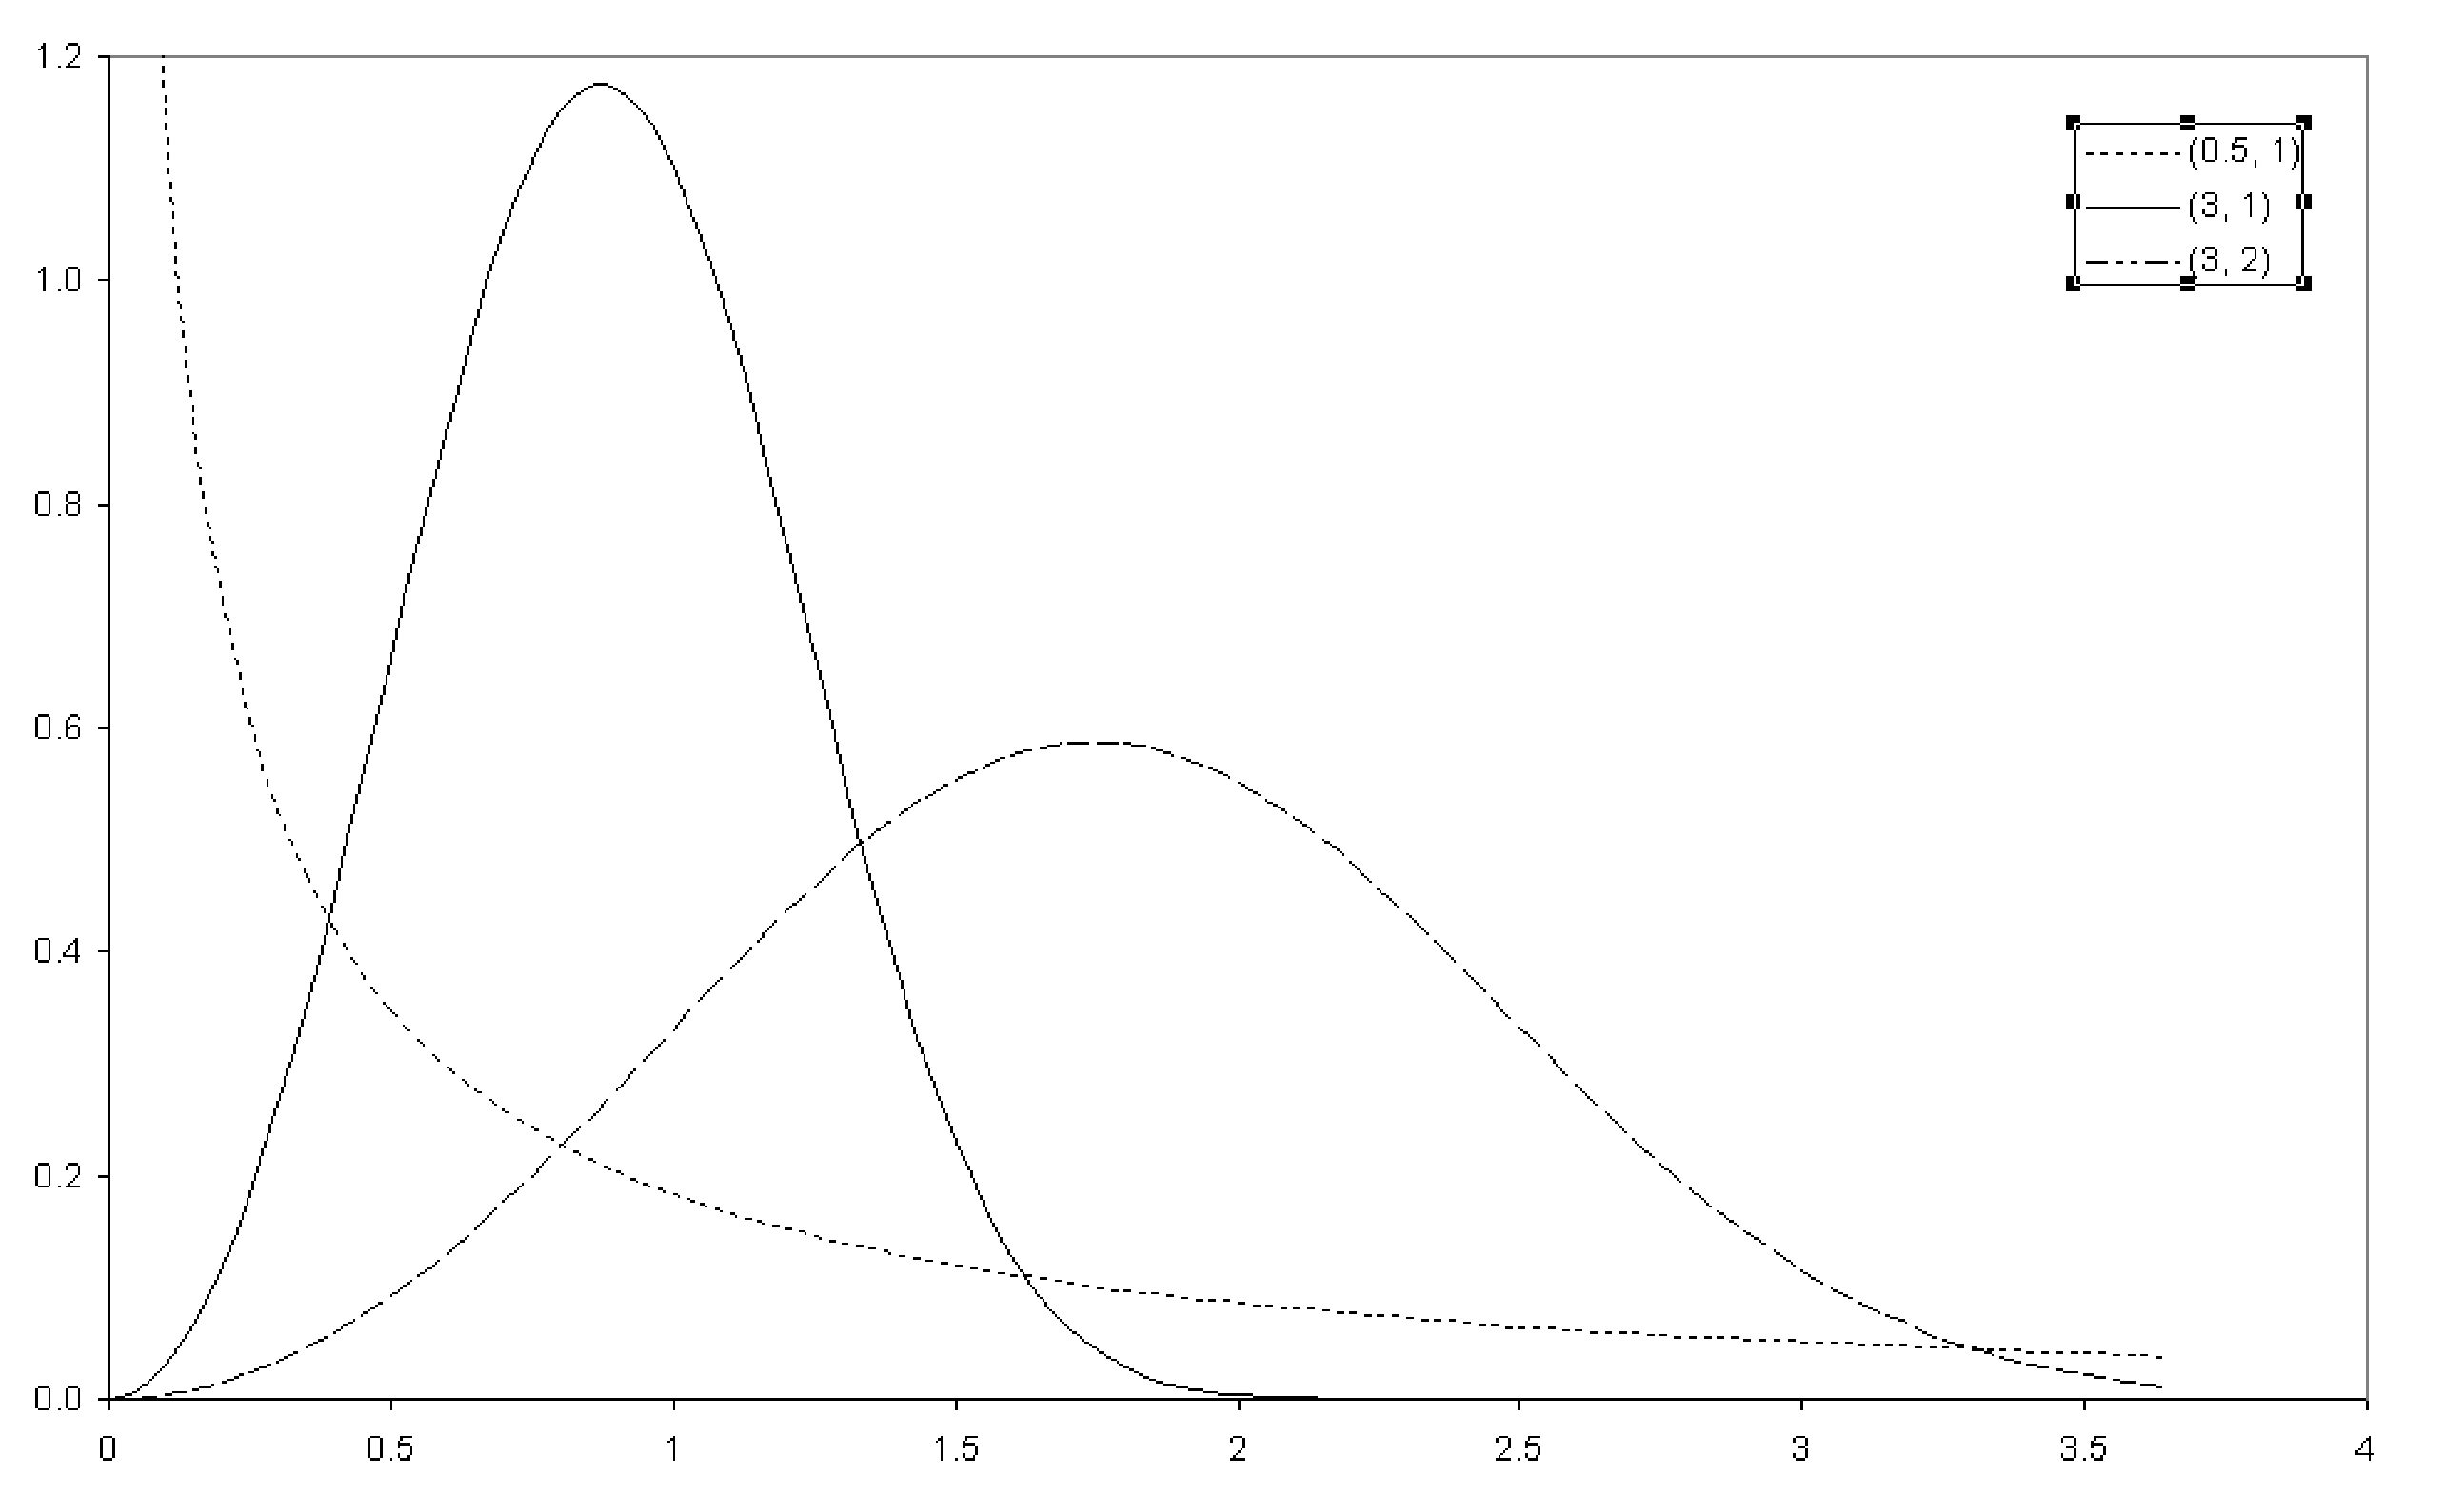
\includegraphics[width=12cm]{Figures/WeibullDistribution}
\caption{Weibull distribution for a few
parameters}\label{fig:weibullDistr}
\end{figure}

Because the Weibull distribution is defined by its distribution
function, the estimation of the initial values of the parameters
from a histogram is made by computing the distribution function at
2 positions. These positions are determined using the histogram
limits and the average so that the estimation of the distribution
function using the histogram has enough significance.

\subsection{Weibull distribution --- Smalltalk  implementation}
\label{sec:weibull} Listing \ref{ls:weibulldist} shows the
implementation of the Weibull distribution in Smalltalk.

\begin{listing} Smalltalk implementation of the Weibull distribution \label{ls:weibulldist}
$$\halign{ #\hfil&\quad#\hfil\cr {\sl Class}& {\Large\bf DhbWeibullDistribution}\cr
{\sl Subclass of }&{\tt DhbProbabilityDensity}\cr\noalign{\vskip 1ex}

{\sl Instance variable names:}&\parbox[t]{4 in}{\tt  alpha beta norm }\cr\noalign{\vskip 1ex}}$$


Class methods
{\parskip 1ex\par\noindent}
{\bf distributionName}
\begin{verbatim}
    ^'Weibull distribution'

\end{verbatim}
{\bf fromHistogram:} {\tt aHistogram}
\begin{verbatim}
    | average xMin xMax accMin accMax |
    aHistogram minimum < 0
        ifTrue: [ ^nil].
    average := aHistogram average.
    xMin := ( aHistogram minimum + average) / 2.
    accMin := ( aHistogram countsUpTo: xMin) / aHistogram totalCount.
    xMax := ( aHistogram maximum + average) / 2.
    accMax := ( aHistogram countsUpTo: xMax) / aHistogram totalCount.
    ^[self solve: xMin acc: accMin upper: xMax acc: accMax]
            when: ExAll do: [ :signal | signal exitWith: nil]

\end{verbatim}
{\bf new}
\begin{verbatim}
    ^self error: 'Illegal creation message for this class'

\end{verbatim}
{\bf shape:} {\tt aNumber1} {\bf scale:} {\tt aNumber2}
\begin{verbatim}
    ^super new initialize: aNumber1 scale: aNumber2

\end{verbatim}
{\bf solve:} {\tt lowX} {\bf acc:} {\tt lowAcc} {\bf upper:} {\tt highX} {\bf acc:} {\tt highAcc}
\begin{verbatim}
    | lowLnAcc highLnAcc deltaLnAcc lowLnX highLnX |
    lowLnAcc := (1 - lowAcc) ln negated ln.
    highLnAcc := (1 - highAcc) ln negated ln.
    deltaLnAcc := highLnAcc - lowLnAcc.
    lowLnX := lowX ln.
    highLnX := highX ln.
    ^self shape: deltaLnAcc / (highLnX - lowLnX)
        scale: ((highLnAcc * lowLnX - (lowLnAcc * highLnX)) / 
                                                       deltaLnAcc) exp

\end{verbatim}



Instance methods
{\parskip 1ex\par\noindent}
{\bf acceptanceBetween:} {\tt aNumber1} {\bf and:} {\tt aNumber2}
\begin{verbatim}
    ^self privateAcceptanceBetween: aNumber1 and: aNumber2

\end{verbatim}
{\bf average}
\begin{verbatim}
    ^(1 / alpha) gamma * beta / alpha

\end{verbatim}
{\bf changeParametersBy:} {\tt aVector}
\begin{verbatim}
    alpha := alpha + ( aVector at: 1).
    beta := beta + ( aVector at: 2).
    self computeNorm.

\end{verbatim}
{\bf computeNorm}
\begin{verbatim}
    norm := alpha/ ( beta raisedTo: alpha).

\end{verbatim}
{\bf distributionValue:} {\tt aNumber}
\begin{verbatim}
    ^aNumber > 0
        ifTrue: [ 1 - ( ( ( aNumber / beta) raisedTo: alpha) negated 
                                                                 exp)]
        ifFalse:[ 0]

\end{verbatim}
{\bf initialize:} {\tt aNumber1} {\bf scale:} {\tt aNumber2}
\begin{verbatim}
    ( aNumber1 > 0 and: [ aNumber2 > 0])
        ifFalse: [ self error: 'Illegal distribution parameters'].
    alpha := aNumber1.
    beta := aNumber2.
    self computeNorm.
    ^self

\end{verbatim}
{\bf parameters}
\begin{verbatim}
    ^Array with: alpha with: beta

\end{verbatim}
{\bf privateInverseDistributionValue:} {\tt aNumber}
\begin{verbatim}
    ^( (1 - aNumber) ln negated raisedTo: ( 1 / alpha)) * beta

\end{verbatim}
{\bf value:} {\tt aNumber}
\begin{verbatim}
    ^( ( aNumber / beta) raisedTo: alpha) negated exp * ( aNumber 
                                        raisedTo: ( alpha - 1)) * norm

\end{verbatim}
{\bf variance}
\begin{verbatim}
    ^( beta squared / alpha) * ( (2 / alpha) gamma * 2 - ( (1 / alpha 
                                             ) gamma squared / alpha))

\end{verbatim}


\end{listing}



\ifx\wholebook\relax\else\end{document}\fi
